% ------------------------------------------------------------------
%  LongPhase 2 -- manuscript draft
%  Build:  latexmk -pdf main.tex   (or `make` in this folder)
% ------------------------------------------------------------------
\documentclass[11pt,a4paper]{article}

\usepackage[utf8]{inputenc}
\usepackage[T1]{fontenc}
\usepackage{lmodern}
\usepackage[margin=2.5cm]{geometry}
\usepackage{setspace}
\usepackage{graphicx}
\usepackage{amsmath}
\usepackage{xspace}
\usepackage{xcolor}
\usepackage{lineno}
\usepackage[super,sort&compress,numbers]{natbib}
\usepackage[hidelinks]{hyperref}
\usepackage{url}

\graphicspath{{figures/}}
\bibliographystyle{naturemag}
\setcitestyle{super,open={},close={}}

% ---------- tool names / editorial macros ----------
\newcommand{\toolname}{LongPhase~2\xspace}       % rename here if needed
\newcommand{\gnnname}{LongPhase-GNN\xspace}
\newcommand{\longphase}{LongPhase\xspace}
\newcommand{\whatshap}{WhatsHap\xspace}
\newcommand{\hapcut}{HapCUT2\xspace}
\newcommand{\methphaser}{MethPhaser\xspace}
\newcommand{\todo}[1]{\textcolor{red}{[#1]}}     % items to verify before submission

% Title (Nature style: declarative, no colon, states the advance and its consequence).
% Alternatives:
%  (a) Learned phase-error detection enables accurate co-phasing of variants and methylation from long reads
%  (b) LongPhase 2 co-phases genetic and epigenetic variation and detects unreliable haplotype assignments
%  (c) Evidence calibration and learned error detection yield accurate long-read haplotypes
\title{Uncertainty-aware haplotype phasing of genetic and epigenetic variation from long reads}

\author{%
Jyun-Hong Lin$^{1}$, Yang-Ming Yeh$^{2}$, Yao-Ting Huang$^{1,\ast}$\\[4pt]
\small $^{1}$Department of Computer Science and Information Engineering, National Chung Cheng University, Chiayi, Taiwan\\
\small $^{2}$Department of Computer Science and Engineering, National Sun Yat-sen University, Kaohsiung, Taiwan\\
\small $^{\ast}$Correspondence: ythuang@cs.ccu.edu.tw}
\date{}

\begin{document}
\sloppy
\onehalfspacing
\linenumbers
\maketitle

\begin{abstract}
Long reads allow haplotypes to be phased from a single sample, but read-based phasers weigh every read observation alike, mostly ignore evidence other than single-nucleotide variants and report phase as a binary state, leaving switch errors to pass unnoticed downstream. Here we present \toolname, which co-phases SNVs, small indels, structural variants and allele-specific methylation in one graph, weights each observation by base quality and sequence context, and assigns every phased variant an uncertainty score. A graph neural network then unphases, rather than flips, the variants it predicts to be misphased. On HG002 nanopore data at 10--60$\times$ coverage, scored against a telomere-to-telomere truth set, \toolname makes 2.9- to 4.8-fold fewer switch errors than WhatsHap and HapCUT2 (1.1- to 1.7-fold under GIAB v4.2.1) and runs six- to eightfold faster at 60$\times$; co-phasing lengthens haplotype blocks by 40\%. \toolname is a drop-in replacement for the LongPhase versions embedded in Clair3, ClairS, Severus and EPI2ME.
\end{abstract}

\section*{Introduction}
% ------------------------------------------------------------------
%  Introduction (Nature Methods style: no subsections, ~900 words,
%  superscript numbered citations, ends with a summary of the advance)
% ------------------------------------------------------------------

Haplotype phasing, the assignment of heterozygous variants to their parental chromosomes, is essential for interpreting the diploid human genome\cite{tewhey2011haplotype,snyder2015haplotype}. Whether two variants act in \textit{cis} or in \textit{trans} decides compound heterozygosity in recessive disease\cite{eisfeldt2025clinical,negi2025napu}; allele-specific expression and methylation report imprinting and \textit{cis}-regulatory variation\cite{akbari2023parentoforigin}; and the haplotype context of somatic mutations reveals clonal structure and loss of heterozygosity in tumours\cite{sun2025advances,li2025unraveling}. Long-read sequencing has made read-based phasing practical at clinical and population scale\cite{logsdon2020longread,wenger2019hifi,beyter2021longread,kolmogorov2023scalable,gustafson2024nanopore}: individual reads span tens to hundreds of kilobases, connect distant heterozygous sites directly and carry native base-modification signals, yielding haplotype blocks orders of magnitude longer than short reads allow, without the trios, chromosome-conformation or single-cell strand data that chromosome-scale phasing otherwise requires\cite{ebert2021haplotype,porubsky2021fully,garg2021computational} and without the reference panels on which statistical phasing depends\cite{hofmeister2023shapeit5}.

Read-based phasing is classically formulated as minimum error correction and solved by dynamic programming or graph partitioning, as in \whatshap\cite{patterson2015whatshap,martin2016whatshap}, \hapcut\cite{edge2017hapcut2}, Longshot\cite{edge2019longshot} and Margin\cite{shafin2021margin}, all of which were designed for single-nucleotide variants (SNVs). We previously introduced \longphase\cite{lin2022longphase}, which recasts phasing as a weighted allele graph, resolves haplotypes at chromosome scale and co-phases SNVs with structural variants (SVs)\cite{sedlazeck2018sniffles,smolka2024sniffles2,jiang2020cutesv}. It has since become infrastructure rather than an alternative: it is the phasing and haplotagging engine of the Clair3 variant-caller family\cite{zheng2022clair3,zheng2026accelerated,zheng2025clair3rna}, of the somatic callers ClairS and ClairS-TO\cite{zheng2026clairs,chen2025clairsto} and of DeepVariant local haplotagging\cite{poplin2018deepvariant,kolesnikov2024local}; it supplies the haplotagged alignments consumed by the somatic SV caller Severus\cite{keskus2025severus}; and it is embedded in the Oxford Nanopore EPI2ME and PacBio HiFi production workflows\cite{ont2025wfhuman,pacbio2025hifisomatic}. Downstream studies inherit its phase across cancer evolution, rapid rare-disease diagnostics, imprinting, regulatory fine-mapping and immune-gene typing\cite{gabbutt2025fluctuating,oneill2024longread,diaz2026mdc1,mcauley2026rectal,zalusky2024threehour,smits2025nanopore,laflamme2024diagnostic,iwasaki2025gnas,thomas2025splice,tian2025finemapping,wang2026immune,galvez2026benchmarking,flack2023pallas,mastrorosa2023applications,mahmoud2025hitchhiker,bioinformatics2026primer}, and it is the baseline against which new phasing algorithms are evaluated\cite{holt2024hiphase,battistella2025ralphi,luo2024gcphase,cao2026cutehap}. A systematic phasing error therefore does not stop at the phaser; it propagates silently into every analysis built on it.

Deployment at this scale has exposed three limitations shared by current phasers. First, they are SNV-centric. Small indels, SVs and 5-methylcytosine (5mC) each carry haplotype linkage that SNVs cannot supply, particularly where heterozygosity is low and blocks terminate; yet methylation-aware methods such as NanoMethPhase\cite{akbari2021nanomethphase}, \methphaser\cite{fu2024methphaser} and HapBridge\cite{chen2025hapbridge} operate as post-processing on an SNV phaser's output, joint phasing of small and structural variants has been restricted to high-accuracy HiFi reads\cite{holt2024hiphase}, and no method places all four evidence classes in one model. Second, they weight read evidence uniformly, although the errors that break haplotypes are not uniform: base-calling errors concentrate in homopolymers and tandem repeats, misplaced reads in segmental duplications create spurious linkages, and heterozygous calls in copy-number-altered regions systematically mislead the graph. The result is the switch error, a flip of haplotype assignment within a block that inverts every inference downstream of it, from compound-heterozygosity calls to haplotype-aware somatic detection\cite{zheng2026clairs,keskus2025severus}. Third, they report phase as an essentially binary state. Statistical phasers have long attached a posterior probability to every phased genotype\cite{hofmeister2023shapeit5}, and \hapcut prunes variants whose posterior under its own read-error model falls below a threshold\cite{edge2017hapcut2}; but that posterior is computed by the likelihood that produced the phase, which treats reads as independent and correctly placed and therefore cannot flag the correlated errors that mis-mapped reads and collapsed paralogues introduce, and \whatshap, Margin and \longphase report no confidence at all. A phase resting on many concordant reads is thus indistinguishable from one resting on two conflicting ones. Learning-based phasers\cite{battistella2025ralphi,luo2024gcphase} replace the haplotype-assembly algorithm rather than diagnose its errors, and remain single-class. These limitations have been underestimated because phasers are benchmarked against GRCh38-based Genome in a Bottle (GIAB) truth sets\cite{zook2019giab,wagner2022giab,wagner2022cmrg} that exclude most segmental duplications and satellite sequence\cite{olson2023benchmarking,dwarshuis2024stratifications}, precisely the regions in which uniform evidence weighting fails, whereas the complete diploid assembly of HG002\cite{hansen2026q100,jarvis2022hg002,rhie2023y} now provides a truth set that assesses them\cite{giab2025q100}, much as the complete CHM13 reference did for variant calling\cite{nurk2022t2t,aganezov2022complete}.

Here we present \toolname, which addresses these limitations through two coupled advances (Fig.~\ref{fig:overview}). First, \toolname co-phases SNVs, small indels, SVs and 5mC within a single weighted phasing graph in one pass over the alignments, calling allele-specific methylation directly from modification tags and calibrating every read observation by base quality and by sequence-context reliability, including homopolymer, tandem-repeat and copy-number-aware down-weighting. Second, it attaches to every phased variant a phasing entropy computed from the weighted haplotype votes, and uses that entropy to select sites for an optional graph neural network that combines local attention over the phasing graph\cite{velickovic2018gat,brody2022gatv2} with window-wide attention\cite{vaswani2017attention,rampasek2022gps}. Variants predicted to be misphased are unphased rather than flipped and the affected phase set is split, so that genotypes are preserved and the corrected output can contain no phase that the graph did not support. Together, the entropy and the learned error probability give read-based phasing what genotype quality gives variant calling: a per-variant confidence that is computed from the evidence structure rather than from the phasing model's own likelihood, and that is available for every co-phased variant class. \toolname is a germline phaser and assumes a diploid genome with balanced allele fractions; the tumour setting, in which loss of heterozygosity, aneuploidy, subclonality and normal-cell admixture violate that assumption, is treated separately in two companion manuscripts that extend the \longphase~1 graph to paired tumour--normal and tumour-only somatic haplotyping\cite{ho2025longphases,chen2026longphaseto} and address neither multimodal germline co-phasing nor phase confidence.

On HG002 nanopore R10.4.1 data from 10$\times$ to 60$\times$, \toolname makes three- to fivefold fewer switch errors than \whatshap and \hapcut\todo{verify: $\sim$3--5$\times$ under the T2T-based benchmark with correction; $\sim$1.1--1.3$\times$ under v4.2.1} and lowers Hamming distance under both the GRCh38-based GIAB v4.2.1 and the telomere-to-telomere-based benchmarks, while running six- to eightfold faster\todo{verify from runtime panel; 5--8$\times$ across 30--60$\times$, 6--8$\times$ at 60$\times$}. The divergence between the two truth sets is itself a result: the GRCh38-based benchmark conceals most of the errors that separate the methods. Co-phasing indels, SVs and methylation extends haplotype blocks by up to 70\% beyond the SNV-only limit\todo{verify: N50 $\sim$5.0~Mb vs $\sim$2.9~Mb at 60$\times$}, and the uncertainty module further reduces switch errors in every variant-class combination, with 86--96\% of the calls it unphases being sites that the benchmark does not support as heterozygous\todo{verify}. \toolname is implemented in C++ with the trained network embedded in the binary, requires no additional dependencies, and is a drop-in replacement for the \longphase versions already deployed in Clair3, ClairS, Severus and the EPI2ME workflows, so that longer, more accurate and now self-assessed haplotypes reach those pipelines without any change to their interfaces.


\begin{figure}[p]
  \centering
  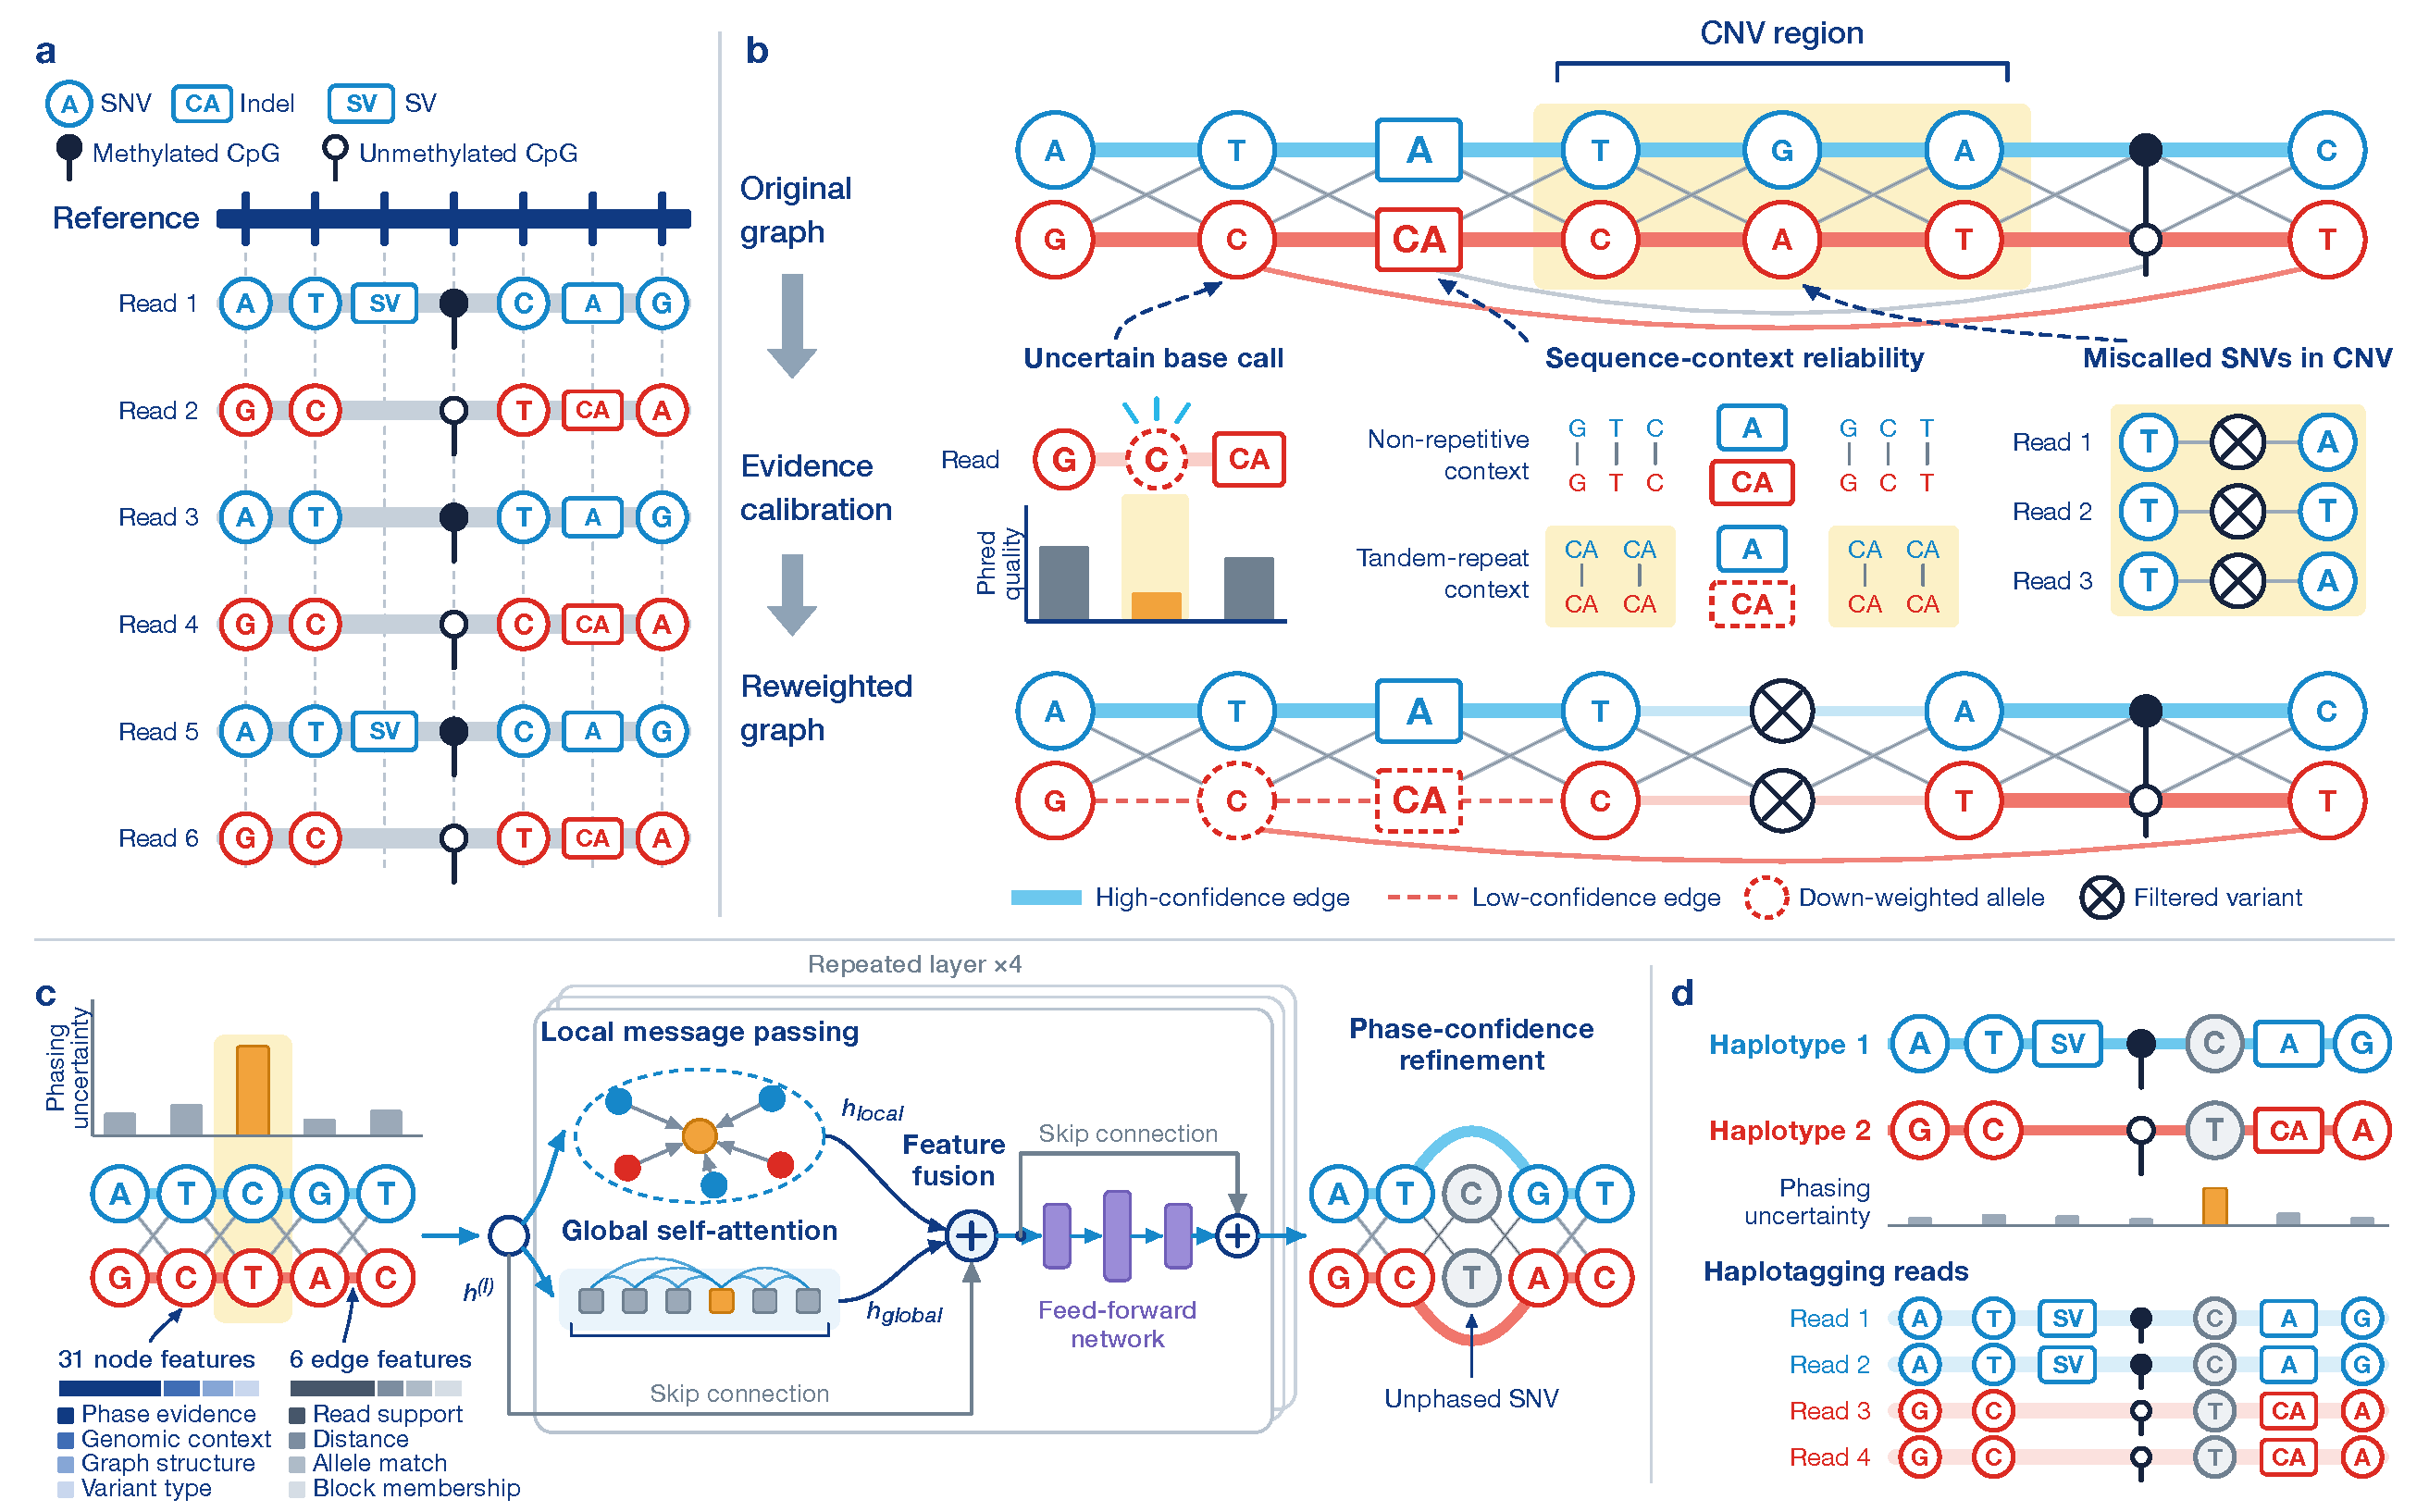
\includegraphics[width=\textwidth]{fig1_overview}
  \caption{\textbf{Overview of \toolname.}
  \textbf{a}, SNVs, small indels, SVs and 5mC sites carried by the same long reads enter one phasing problem; alleles are coloured by read haplotype.
  \textbf{b}, Weighted phasing graph. Read-supported edges link allele nodes, and each observation is weighted by base quality and sequence context; the inset shows an indel down-weighted inside a tandem repeat.
  \textbf{c}, Each variant receives a phasing-uncertainty score (Methods), and a graph neural network (GATv2 and Transformer layers; Supplementary Fig.~6) classifies the variants around the most uncertain ones. Variants predicted to be misphased are unphased (grey), not flipped.
  \textbf{d}, Output: phased haplotypes of all four variant classes with per-variant uncertainty, and haplotagged reads.}
  \label{fig:overview}
\end{figure}

\section*{Results}
% ------------------------------------------------------------------
%  Results (bold run-in subheadings that state
%  the finding, present tense for figure description, past tense for
%  what was done, no methods detail).
%
%  NUMBERS: LongPhase 2 values (SNV-only and four-class, with and
%  without GNN; phased fraction, switch errors, Hamming, N50, indel
%  fraction) were replaced on 2026-09-20 with the exact values from the
%  `longphase compare` tables in "GNN source/sw_*.log" (v5.0q, chr1-22;
%  10x has nine replicates there, seed 10 missing). WhatsHap, HapCUT2,
%  LongPhase 1.0, the SNV+indel/SV/5mC configurations, SV and 5mC phased
%  fractions, runtimes and the v4.2.1 counts are still read from the
%  plots in LongPhaseGNN_0902_2-1.pptx (slides 7-11).
%
%  REPLICATE STRUCTURE: 10--20x = mean of ten down-sampling replicates;
%  30--60x = a single replicate. Every quoted value must carry the
%  corresponding dispersion (10--20x) or a robustness statement (30--60x).
% ------------------------------------------------------------------

\subsection*{\toolname co-phases SNVs, indels, SVs and methylation in one graph and scores every phased variant}
\toolname resolves haplotypes in three stages (Fig.~\ref{fig:overview}). All heterozygous evidence carried by the same long reads, comprising SNVs, small indels, SVs and allele-specific 5mC sites called by the built-in \texttt{modcall} module, enters a single weighted phasing graph per chromosome. Within that graph each observation is calibrated by base quality and by the reliability of its sequence context, so that homopolymers, tandem repeats and copy-number-altered regions contribute less (Fig.~\ref{fig:overview}a,b). A graph neural network then inspects a local window around each phased variant (Fig.~\ref{fig:overview}c). Variants predicted to be misphased are unphased instead of flipped, and any phase set that becomes disconnected is split, so genotypes are preserved and no new phase assignment is ever introduced. The outputs are phased VCFs for every variant class and haplotagged alignments (Fig.~\ref{fig:overview}d).

We evaluated \toolname on HG002 nanopore R10.4.1 whole-genome data down-sampled from 10$\times$ to 60$\times$ coverage (Methods). Throughout, values quoted at 10--20$\times$ are means over ten independent down-sampling replicates, and values quoted at 30--60$\times$ come from a single replicate. Phasing accuracy was scored against two independent truth sets: the GRCh38-based GIAB v4.2.1 benchmark, and the benchmark derived from the complete diploid telomere-to-telomere (T2T) assembly of the same individual, T2T-HG002 (referred to here as v5.0q), which extends evaluation into the segmental duplications, satellite arrays and other difficult regions that v4.2.1 excludes. Unless stated otherwise, results refer to the v5.0q benchmark and to SNVs, the only variant class that all compared tools phase.

\subsection*{\toolname phases SNVs three- to fivefold more accurately and six- to eightfold faster than \whatshap and \hapcut}
On identical Clair3 variant calls and SNV-only phasing, \toolname made several-fold fewer switch errors than \whatshap~2.8 and \hapcut~1.3.4 at every coverage (Fig.~\ref{fig:snv}). Without the neural network, the switch error rate of \toolname was 0.046\% at 30$\times$ and 0.034\% at 60$\times$, against approximately 0.115\% and 0.085\% for \whatshap and 0.15\% and 0.11\% for \hapcut, a 2.5-fold reduction relative to \whatshap and a 3.2-fold reduction relative to \hapcut (Fig.~\ref{fig:snv}b)\todo{\whatshap and \hapcut rates are still read from the plots (the \toolname values are now exact, from the \texttt{compare} tables); the two fold-changes are averages over 30--60$\times$ (\whatshap 2.6$\times$ at 30$\times$ and 2.4$\times$ at 60$\times$; \hapcut 3.3$\times$ and 3.1$\times$); decide whether to quote ranges instead, as elsewhere in this section}. Correction reduced the rate further, to 0.031\% at 30$\times$ and 0.023\% at 60$\times$, so that \toolname with correction made 3.6--3.9-fold fewer switch errors than \whatshap and 4.7--5.0-fold fewer than \hapcut across 30--60$\times$, and 2.6-fold and 3.1-fold fewer at 10$\times$\todo{quote the \whatshap and \hapcut switch error rates at 10$\times$ (approximately 0.225\% and 0.27\%) so that the 2.6- and 3.1-fold claims are verifiable from the reported numbers}. In absolute terms correction helped most where evidence is sparsest: at 10$\times$ the rate fell by 0.039 percentage points, from 0.121\% to 0.082\%, against 0.015 percentage points at 30$\times$ and 0.011 at 60$\times$; in relative terms the reduction was close to one-third at every coverage (31--34\%). The block-wise Hamming distance, which counts misassigned variants rather than switch points and therefore penalizes long-range flips, showed the same ordering: at 30$\times$ the distance was approximately 2.6\% for \whatshap and \hapcut, 2.4\% for \toolname and 1.8\% after correction, and at 10$\times$ the distance fell from 7.7--7.8\% for the two competing tools to 5.3\% after correction (Fig.~\ref{fig:snv}c).

This gain in accuracy did not cost completeness or haplotype length. All tools phased a similar fraction of benchmark heterozygous SNVs, rising from roughly 78\% at 10$\times$ to a plateau above 91\% from 20$\times$ onwards, with \whatshap phasing about one percentage point more than \toolname at every coverage (approximately 92.5\% versus 91.4--91.6\% at 30--60$\times$), consistent with the more conservative read-based correction of \toolname (Fig.~\ref{fig:snv}a). Block N50 grew almost linearly with coverage for all tools and was highest for \toolname (approximately 2.9~Mb at 60$\times$, versus 2.75~Mb for \whatshap and \hapcut); the neural network shortened blocks by 5--9\% at 10--20$\times$ (0.84~Mb versus 0.92~Mb at 10$\times$) and by less than 3\% from 30$\times$ onwards (2.86 versus 2.91~Mb at 60$\times$) (Fig.~\ref{fig:snv}d). \toolname was also substantially faster: whole-genome phasing took 3~min at 10$\times$ and 15~min at 60$\times$, compared with 26 and 95~min for \hapcut and 26 and 115~min for \whatshap, a 6--8-fold speed-up at 60$\times$ (5--8-fold across 30--60$\times$); the neural network added 1--2~min (Fig.~\ref{fig:snv}e)\todo{threads and hardware; exact times, including the 30$\times$ times (approximately 12, 65 and 90~min); add peak memory alongside runtime in a Supplementary table, which Methods states was recorded}.

\subsection*{A telomere-to-telomere benchmark exposes switch errors hidden by the GRCh38 truth set}
Scoring the same phased VCFs against the two truth sets changed the apparent separation between methods by more than fourfold (Fig.~\ref{fig:benchmarks}). Under GIAB v4.2.1, all methods converged to a narrow band of 1,600--2,200 switch errors genome-wide from 30$\times$ upwards, with corrected \toolname lowest (approximately 1,650), followed by uncorrected \toolname (1,700), \whatshap (1,800), \longphase~1.0 (2,000) and \hapcut (2,100) (Fig.~\ref{fig:benchmarks}b)\todo{exact counts}. Under v5.0q the same VCFs separated four to five times more widely: at 60$\times$ \hapcut made approximately 2,330 switch errors, \whatshap 1,790, \longphase~1.0 1,380, \toolname 743 and \toolname with correction 496, and at 10$\times$ the corresponding counts were 5,030, 4,390, 4,030, 2,258 and 1,517 (Fig.~\ref{fig:benchmarks}c).

Metrics other than the error counts separate the five methods far less. The fraction of benchmark heterozygous SNVs phased (Fig.~\ref{fig:benchmarks}a) and the phase-block N50 (Fig.~\ref{fig:benchmarks}d), which is benchmark independent, differ little between methods\todo{quote the phased fraction and N50 of \longphase~1.0 at 10$\times$ and 60$\times$ (approximately 65\% and 92\%; 0.55 and 2.85~Mb); \longphase~1.0 appears only in Fig.~\ref{fig:benchmarks} and is currently never described quantitatively for these two panels}. Hamming distance was also nearly identical under the two benchmarks for \hapcut, \whatshap and \toolname with and without correction (Fig.~\ref{fig:benchmarks}e,f), indicating that the additional v5.0q switch errors are mostly isolated switches rather than long-range flips. \longphase~1.0 was the exception. Despite an intermediate number of switch errors, \longphase~1.0 showed a Hamming distance of 6--12\% under both benchmarks, which points to long-range flips within blocks. The read-based correction and copy-number-aware filtering introduced in \toolname remove these.

\subsection*{Co-phasing indels, SVs and methylation lengthens blocks by up to 75\% but raises the SNV switch error rate}
Joint phasing of all four variant classes extended haplotypes well beyond the SNV-only limit, at a measurable cost in SNV accuracy that correction then more than recovered (Figs.~\ref{fig:cophasing} and~\ref{fig:combinations}). Indels and methylation sites provide new links across SNV-poor regions, so block N50 at 60$\times$ increased from approximately 2.9~Mb for SNV-only phasing to 4.3~Mb with indels, to 3.1~Mb with methylation alone and to 5.1~Mb with all four classes (Fig.~\ref{fig:combinations}, right column). At the same time, indel observations are noisier than SNV observations: the SNV switch error rate of uncorrected co-phasing rose from 0.034\% (SNV only) to 0.043\% (all classes) at 60$\times$ and from 0.121\% to 0.154\% at 10$\times$, while the Hamming distance rose from 1.8\% to 7.2\% at 60$\times$ (Fig.~\ref{fig:cophasing}e,f). Decomposing the combinations showed that indels carry almost all of the additional error. SNV+SV and SNV+methylation had switch error rates and Hamming distances indistinguishable from SNV-only phasing, while SNV+indel matched the four-class configuration (Fig.~\ref{fig:combinations}).

Adding classes did not make the phasing of any single class less complete. The fraction of phased SNVs was unchanged relative to SNV-only phasing (Fig.~\ref{fig:cophasing}a). The fraction of benchmark heterozygous indels that were phased rose from 31\% at 10$\times$ to 45\% at 60$\times$ and was unaffected by the neural network (Fig.~\ref{fig:cophasing}b)\todo{clarify denominator: all GIAB indels or those called by Clair3}. Of the allele-specific 5mC sites identified by \texttt{modcall}, more than 99\% were phased at every coverage, and the neural network unphased 1.5--5\% of those sites, mostly at low coverage (Fig.~\ref{fig:cophasing}c). Roughly 68--70\% of heterozygous SVs called by Sniffles2 were phased, decreasing slightly with coverage as more low-support SVs were called, and correction removed a further 2 percentage points (Fig.~\ref{fig:cophasing}d).

\todo{Two comparisons are missing from this section and will be requested. (i) \methphaser, which Methods states was run in the methylation-assisted setting, is never reported: add the SNV+5mC comparison of \toolname against \whatshap followed by \methphaser (block N50, switch error rate, Hamming distance) or remove \methphaser from Methods. (ii) \longphase~1.0 already co-phases SNVs with SVs, so the SNV+SV and four-class configurations should be compared against it to separate the contribution of the new evidence classes from that of the new evidence calibration; \longphase~1.0 currently appears only in Fig.~\ref{fig:benchmarks}. Also report the phasing accuracy, not only the phased fraction, of the indels, SVs and 5mC sites themselves (indels and SVs against the v5.0q and GIAB SV benchmarks; 5mC against imprinted differentially methylated regions, for which parent-of-origin is known).}

\subsection*{Neural-network correction reduces switch errors in every variant-class configuration}
The neural network reduced the SNV switch error rate in all five configurations and at every coverage (Fig.~\ref{fig:combinations}, left column). For SNV-only phasing the rate fell by about one-third at every coverage (31--34\%; for example from 0.034\% to 0.023\% at 60$\times$); for all four classes it fell by 37--40\%, from 0.043\% to 0.027\% at 60$\times$ and from 0.154\% to 0.093\% at 10$\times$, and SNV+indel behaved alike. Corrected co-phasing was therefore more accurate than uncorrected SNV-only phasing at every coverage (Fig.~\ref{fig:cophasing}e) while retaining substantially longer blocks (Fig.~\ref{fig:combinations}, right column). The correction was even more effective on the Hamming distance of indel-containing configurations, which fell from 7.2\% to 3.3\% at 60$\times$ and from 11.0\% to 7.0\% at 10$\times$ (Fig.~\ref{fig:combinations}, middle column), which suggests that a large share of the indel-induced errors are long-range flips the network recognizes from the surrounding vote structure. The price was a moderate reduction in block N50 for indel-containing configurations, from 4.3~Mb to 3.7~Mb (SNV+indel) and from 5.1~Mb to 4.1~Mb (all classes) at 60$\times$, because unphased variants that bridged two blocks split those blocks. For configurations without indels the N50 was almost unchanged. On balance, co-phasing remains worthwhile: even after correction, four-class co-phasing yielded blocks approximately 40\% longer than SNV-only phasing at 60$\times$, together with a lower switch error rate than uncorrected SNV-only phasing.

\todo{Ablations a reviewer will demand for this section: (i) the network versus the simple baseline it replaces, namely unphasing every variant with PE above a fixed threshold, matched for the number of variants unphased (this is the control for the claim made in the next section that a fixed entropy threshold cannot substitute for the network); (ii) sensitivity of all metrics to the break threshold (0.30) and to the PE trigger threshold (0.8), ideally as a switch-error-versus-N50 trade-off curve; (iii) precision and recall of the network on held-out switch-error labels. Also state explicitly, here or in Methods, which HG002 chromosomes and coverages were held out of training, since training and evaluation use the same individual.}

\subsection*{Unphased variants are predominantly unsupported heterozygous calls}
To see what the network actually removes, we classified every SNV that \toolname phased and the network subsequently unphased (SNV-only phasing, single replicate, seed 1) against the v5.0q benchmark (Fig.~\ref{fig:unphased}). The network unphased approximately 60,000 SNVs at every coverage, but 86--96\% of those SNVs were calls that the benchmark does not support as heterozygous, either because the site is absent from the benchmark (80--94\%) or because the benchmark calls the site homozygous. Only 4.0\% (2,411 variants) at 60$\times$ and 14\% at 10$\times$ were genuine heterozygous sites (Fig.~\ref{fig:unphased}a). Little real phasing information is therefore lost.

Cross-tabulating each unphased variant by read depth and by phasing informativeness, the number of informative reads linking each variant to its neighbours, showed that genuine heterozygotes were removed overwhelmingly at normal depth with weak phasing evidence (61--81\%), whereas benchmark-absent calls shifted towards low depth as coverage increased (12.5\% at 10$\times$ to 58.6\% at 60$\times$), as expected in hard-to-map regions where reads are lost to alternative loci (Fig.~\ref{fig:unphased}b). High depth alone never caused a variant to be unphased. Among the genuine heterozygotes that were removed, 43\% at 10$\times$ had unanimous but sparse haplotype votes, compared with 17\% of benchmark-absent calls, and this share fell to 22\% at 60$\times$ as evidence accumulated; a further 21--25\% of genuine heterozygotes and 16--18\% of benchmark-absent calls had near-equivocal votes at every coverage (Fig.~\ref{fig:unphased}c)\todo{PE $\ge 0.8$ prevalences read from Fig.~\ref{fig:unphased}c; replace with exact values}. The vote balance at the variant itself would therefore have missed most of the removed heterozygotes; the network, which sees the votes of all neighbours in the window, did not. Clustering within 50~bp and low genotype quality, by contrast, were present in 46--49\% of benchmark-absent calls at every coverage and were far less frequent among genuine heterozygotes, which marks those calls as variant-caller artefacts rather than phasing failures.

Correction therefore loses little true phasing information, about 2,400 SNVs at 60$\times$ out of 2.19 million phased benchmark SNVs\todo{the \texttt{compare} tables put the loss of phased benchmark SNVs at 60$\times$ at 2,055 (2,193,366 before, 2,191,311 after correction), against the 2,411 genuine heterozygotes counted in Fig.~6a; reconcile the two definitions}. Most removals are false heterozygous calls whose spurious phase would otherwise propagate into haplotagged reads and downstream haplotype-aware callers.

\todo{Generalization experiments missing from the Results as a whole, each of which a reviewer is likely to require, and none of which may be asserted without data: (i) a second individual, e.g.\ HG001 or HG005, to show that the network does not encode HG002-specific structure (the model was trained on HG002 and every result above is on HG002); (ii) PacBio HiFi data, since the Discussion claims the graph algorithm supports both platforms and the Introduction contrasts \toolname with HiFi-restricted joint phasing; (iii) a runtime and peak-memory table across coverages, variant-class configurations and thread counts, covering \toolname, \whatshap, \hapcut and \longphase~1.0; (iv) a demonstration that improved phase propagates downstream, e.g.\ haplotagging accuracy or haplotype-aware variant calling, which the Discussion asserts as the motivation for the work.}

\todo{Item (iv) above may already be done. The group's algorithm slides contain a ClairS somatic-calling experiment across six tumour cell lines (COLO829, H1437, H2009, HCC1395, HCC1937, HCC1954) at five simulated purities (20--100\%), in which the germline phaser supplying the haplotagged alignments is varied between \whatshap~2.4, \longphase~1.7.3 and \longphase~2.0 and everything downstream is held fixed. This is exactly the downstream-impact result the Discussion promises, and it is the strongest available answer to ``does a lower switch error rate actually matter?'': on HCC1395 at 100\% purity, somatic SNV F1 rises from 0.8250 with \longphase~1.7.3 to 0.8398 with \longphase~2.0, with the margin widening at low purity. The experiment must be re-run before it can be used: the ``\longphase~2.0'' in those slides is a pre-release build of the 1.7.3 era, not the version submitted here, so its numbers do not describe the method reported in this paper and the improvement may be larger or smaller once repeated. Three further caveats: the comparison against \whatshap was mixed rather than uniformly favourable, so the claim should be framed as ``improves on the \longphase version ClairS currently embeds'' rather than as a win over all phasers; the experiment uses ClairS v0.4.0 in \texttt{ssrs} mode, which must be stated; and this is germline phasing evaluated by its effect on somatic calling, which must be framed so that it is not read as a somatic-phasing claim. The experimental design, however, is sound and directly reusable: hold the somatic caller fixed, vary only the germline phaser supplying the haplotagged alignments, and sweep purity.}

\todo{The same slides contain an HG002 germline comparison whose numbers differ substantially from Fig.~2 (switch error rate nearly flat at 0.056\% from 10$\times$ to 60$\times$, against 0.125\% falling to 0.035\% here). The configurations differ in every respect (DeepVariant v1.9.0 instead of Clair3, the GIAB benchmark instead of v5.0q, \whatshap~2.4 instead of 2.8, and a pre-release build instead of the submitted version), so the two are not comparable and the slide figures must not be mixed into this manuscript. Separately, confirm which \longphase~1 release is the baseline in Fig.~3: the text says 1.0, the slides used 1.7.3, and the two are different programs. Whichever was run, give its exact version and commit in Methods.}


\begin{figure}[p]
  \centering
  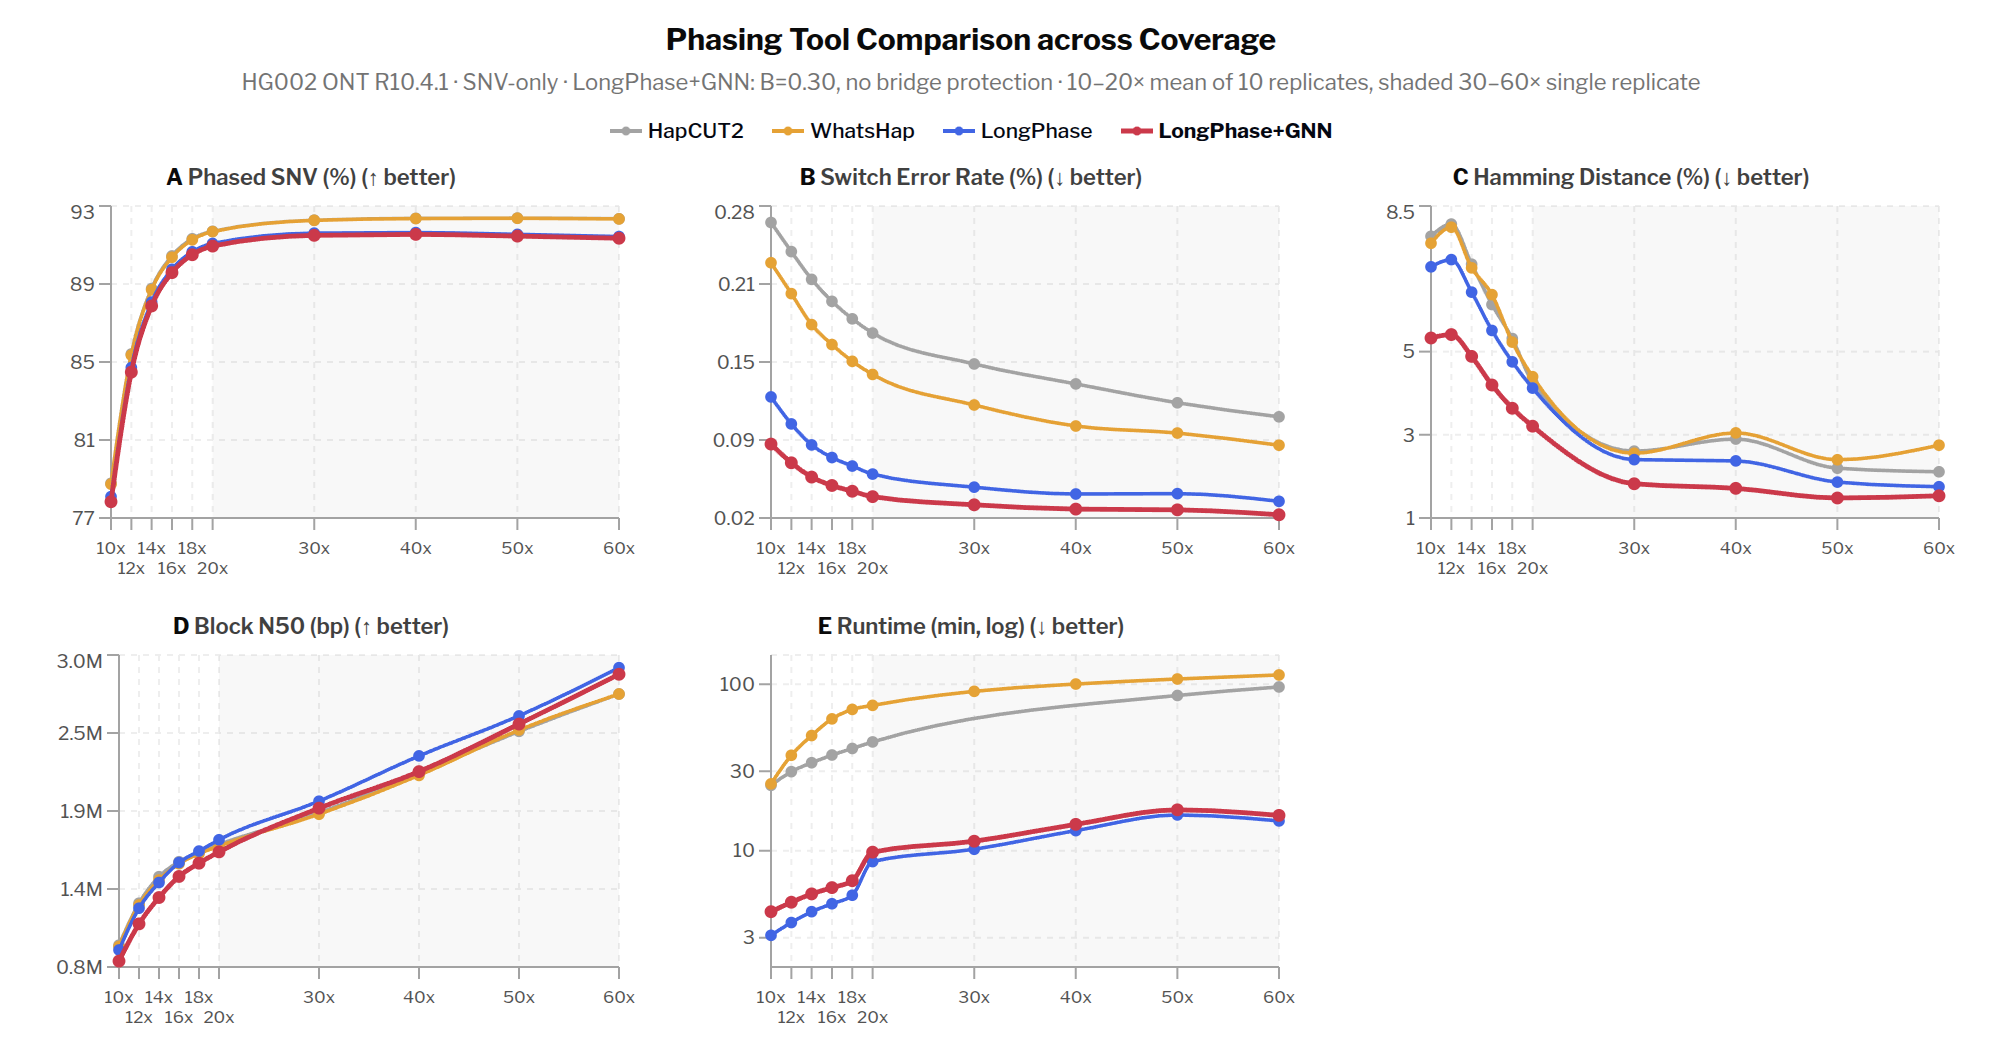
\includegraphics[width=\textwidth]{fig2_snv_comparison}
  \caption{\textbf{SNV phasing accuracy, block length and runtime compared with WhatsHap and HapCUT2.}
  HG002 nanopore R10.4.1 reads down-sampled to 10--60$\times$; SNV-only phasing of identical Clair3 calls; scored against the benchmark derived from the complete diploid T2T-HG002 assembly (v5.0q). Points at 10--20$\times$ are means of independent down-sampling replicates ($n=10$, except $n=9$ at 10$\times$ for \toolname); the shaded region (30--60$\times$) is a single replicate.
  \textbf{a}, Fraction of benchmark heterozygous SNVs phased.
  \textbf{b}, Switch error rate.
  \textbf{c}, Block-wise Hamming distance.
  \textbf{d}, Phase-block N50.
  \textbf{e}, Wall-clock runtime (log scale, \todo{$t$} threads, whole genome); \toolname with correction includes the neural-network stage.
  Grey, HapCUT2 1.3.4; orange, WhatsHap 2.8; blue, \toolname; red, \toolname with neural-network correction.}
  \label{fig:snv}
\end{figure}

\begin{figure}[p]
  \centering
  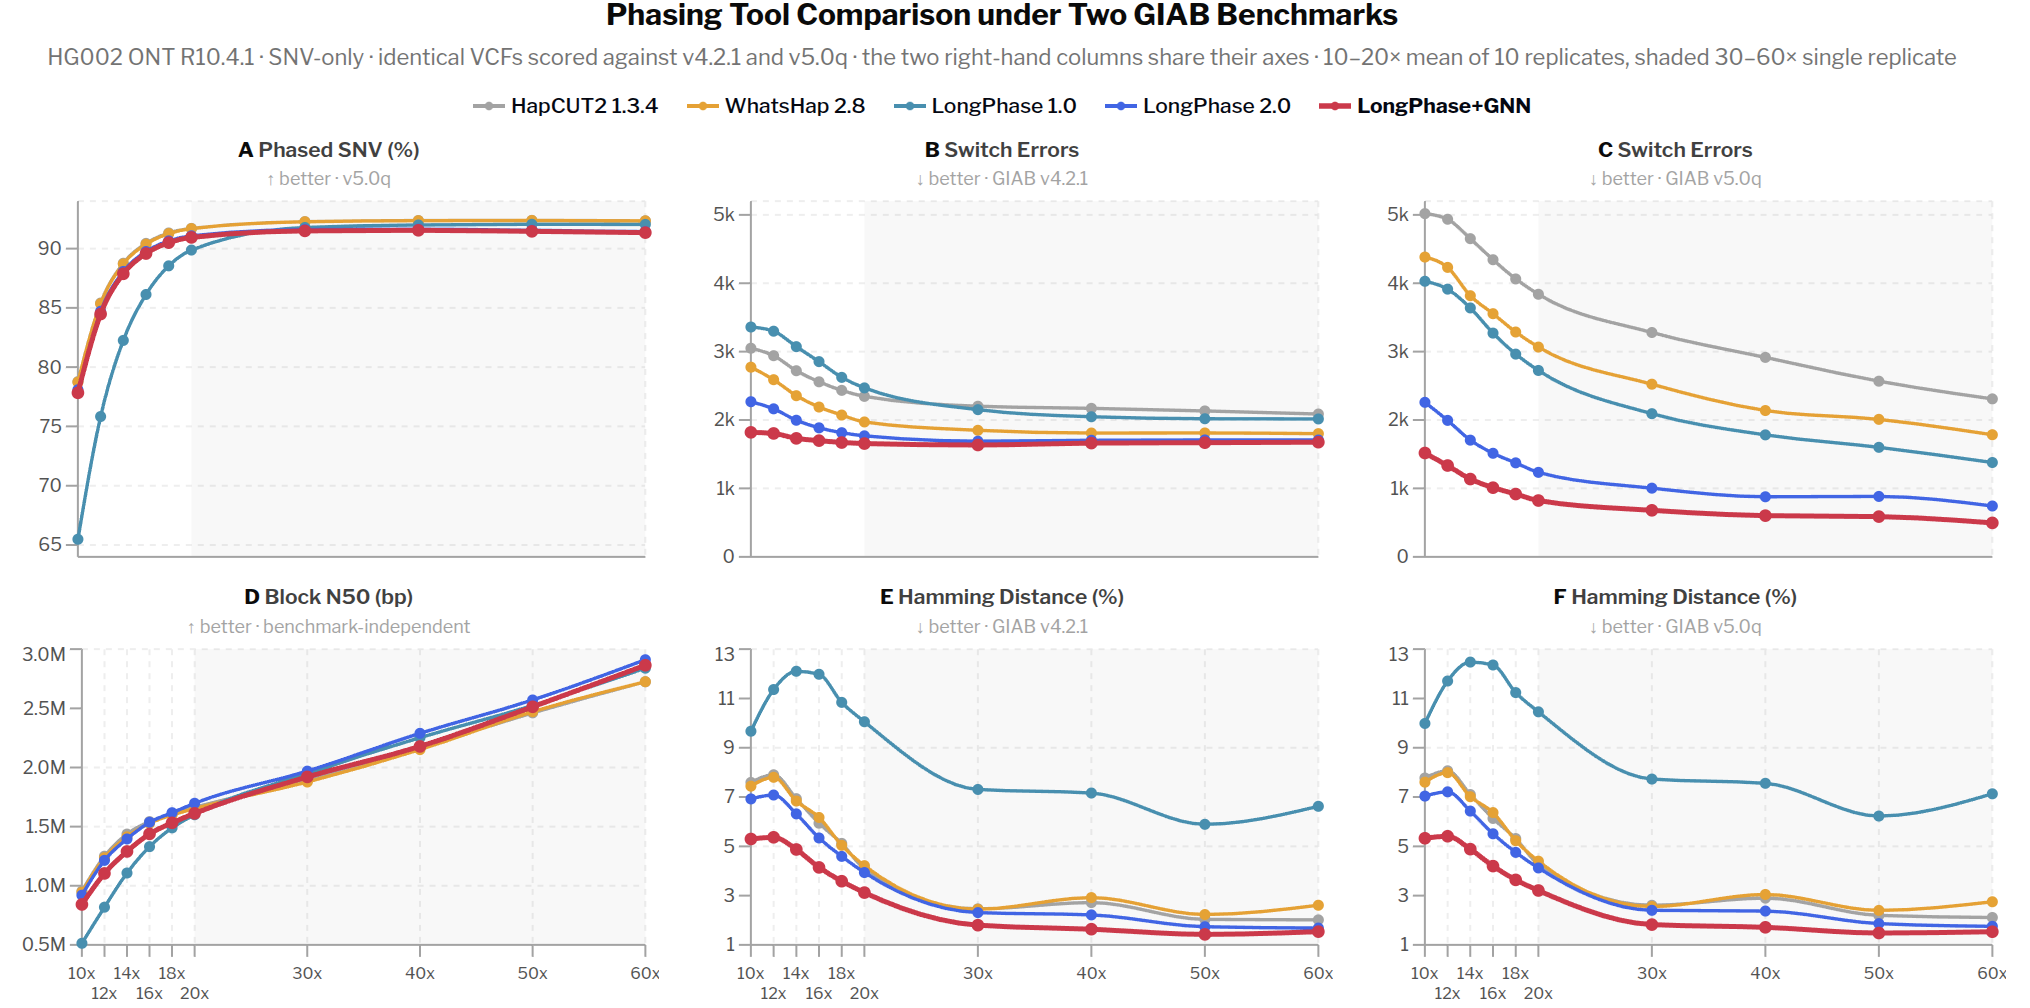
\includegraphics[width=\textwidth]{fig3_two_benchmarks}
  \caption{\textbf{The same phased VCFs scored against the GRCh38-based GIAB v4.2.1 and the T2T-HG002-derived v5.0q benchmarks.}
  SNV-only phasing of HG002 nanopore R10.4.1 data; replicates as in Fig.~\ref{fig:snv}. Only the truth set differs between the two columns; v5.0q additionally assesses the segmental duplications, satellite arrays and other repeat-rich sequence that v4.2.1 excludes.
  \textbf{a}, Fraction of benchmark heterozygous SNVs phased (v5.0q).
  \textbf{b},\textbf{c}, Genome-wide switch-error counts under v4.2.1 (\textbf{b}) and v5.0q (\textbf{c}); the two panels share axes.
  \textbf{d}, Phase-block N50 (benchmark independent).
  \textbf{e},\textbf{f}, Hamming distance under v4.2.1 (\textbf{e}) and v5.0q (\textbf{f}).
  Grey, HapCUT2 1.3.4; orange, WhatsHap 2.8; teal, \longphase~1.0; blue, \toolname; red, \toolname with neural-network correction.}
  \label{fig:benchmarks}
\end{figure}

\begin{figure}[p]
  \centering
  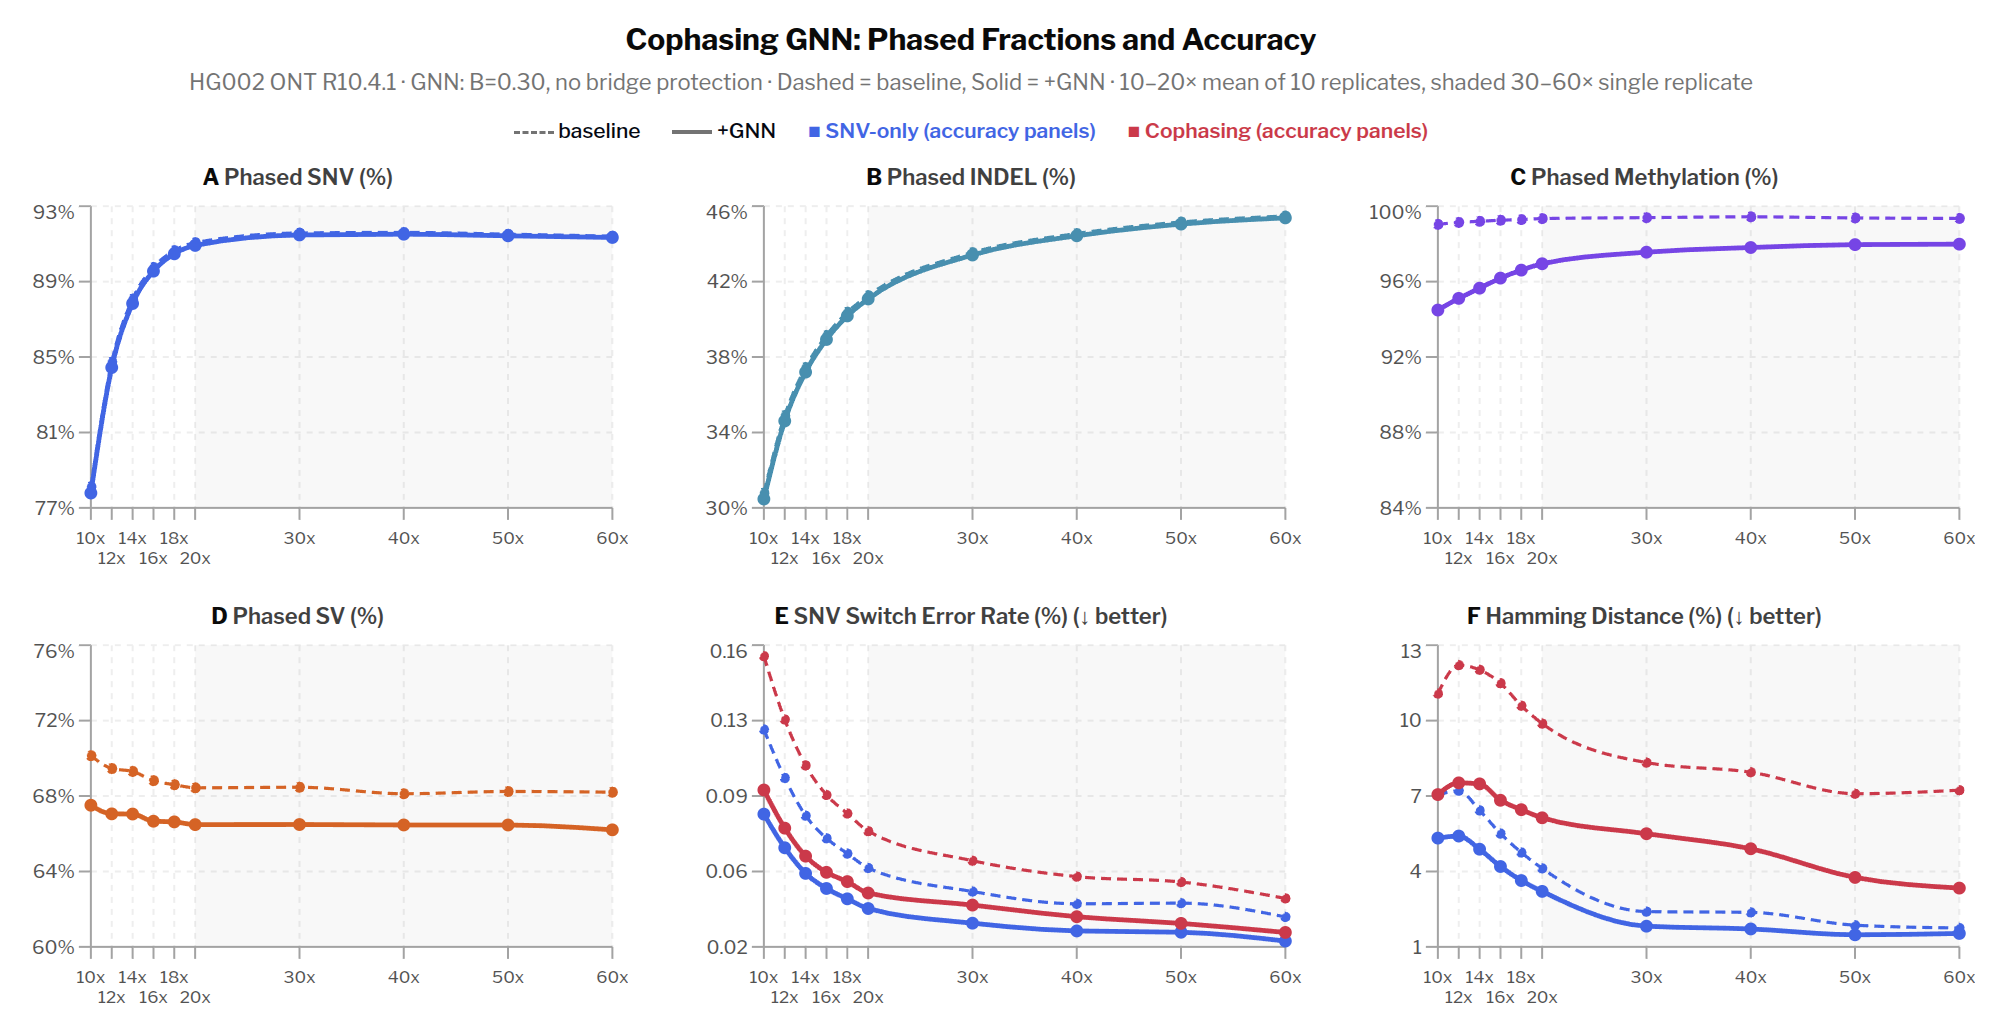
\includegraphics[width=\textwidth]{fig4_cophasing}
  \caption{\textbf{Co-phasing of SNVs, indels, SVs and allele-specific methylation.}
  HG002 nanopore R10.4.1 data, 10--60$\times$; replicates as in Fig.~\ref{fig:snv}; dashed lines, \toolname; solid lines, \toolname with neural-network correction.
  \textbf{a}--\textbf{d}, Fraction of phased SNVs (\textbf{a}), indels (\textbf{b}), allele-specific 5mC sites (\textbf{c}) and SVs (\textbf{d}) in the four-class co-phasing configuration.
  \textbf{e},\textbf{f}, SNV switch error rate (\textbf{e}) and Hamming distance (\textbf{f}) for SNV-only phasing (blue) and four-class co-phasing (red), each with (solid) and without (dashed) correction. Denominators: GIAB v5.0q heterozygous SNVs and indels; Sniffles2 heterozygous SVs; \texttt{modcall} heterozygous 5mC sites.}
  \label{fig:cophasing}
\end{figure}

\begin{figure}[p]
  \centering
  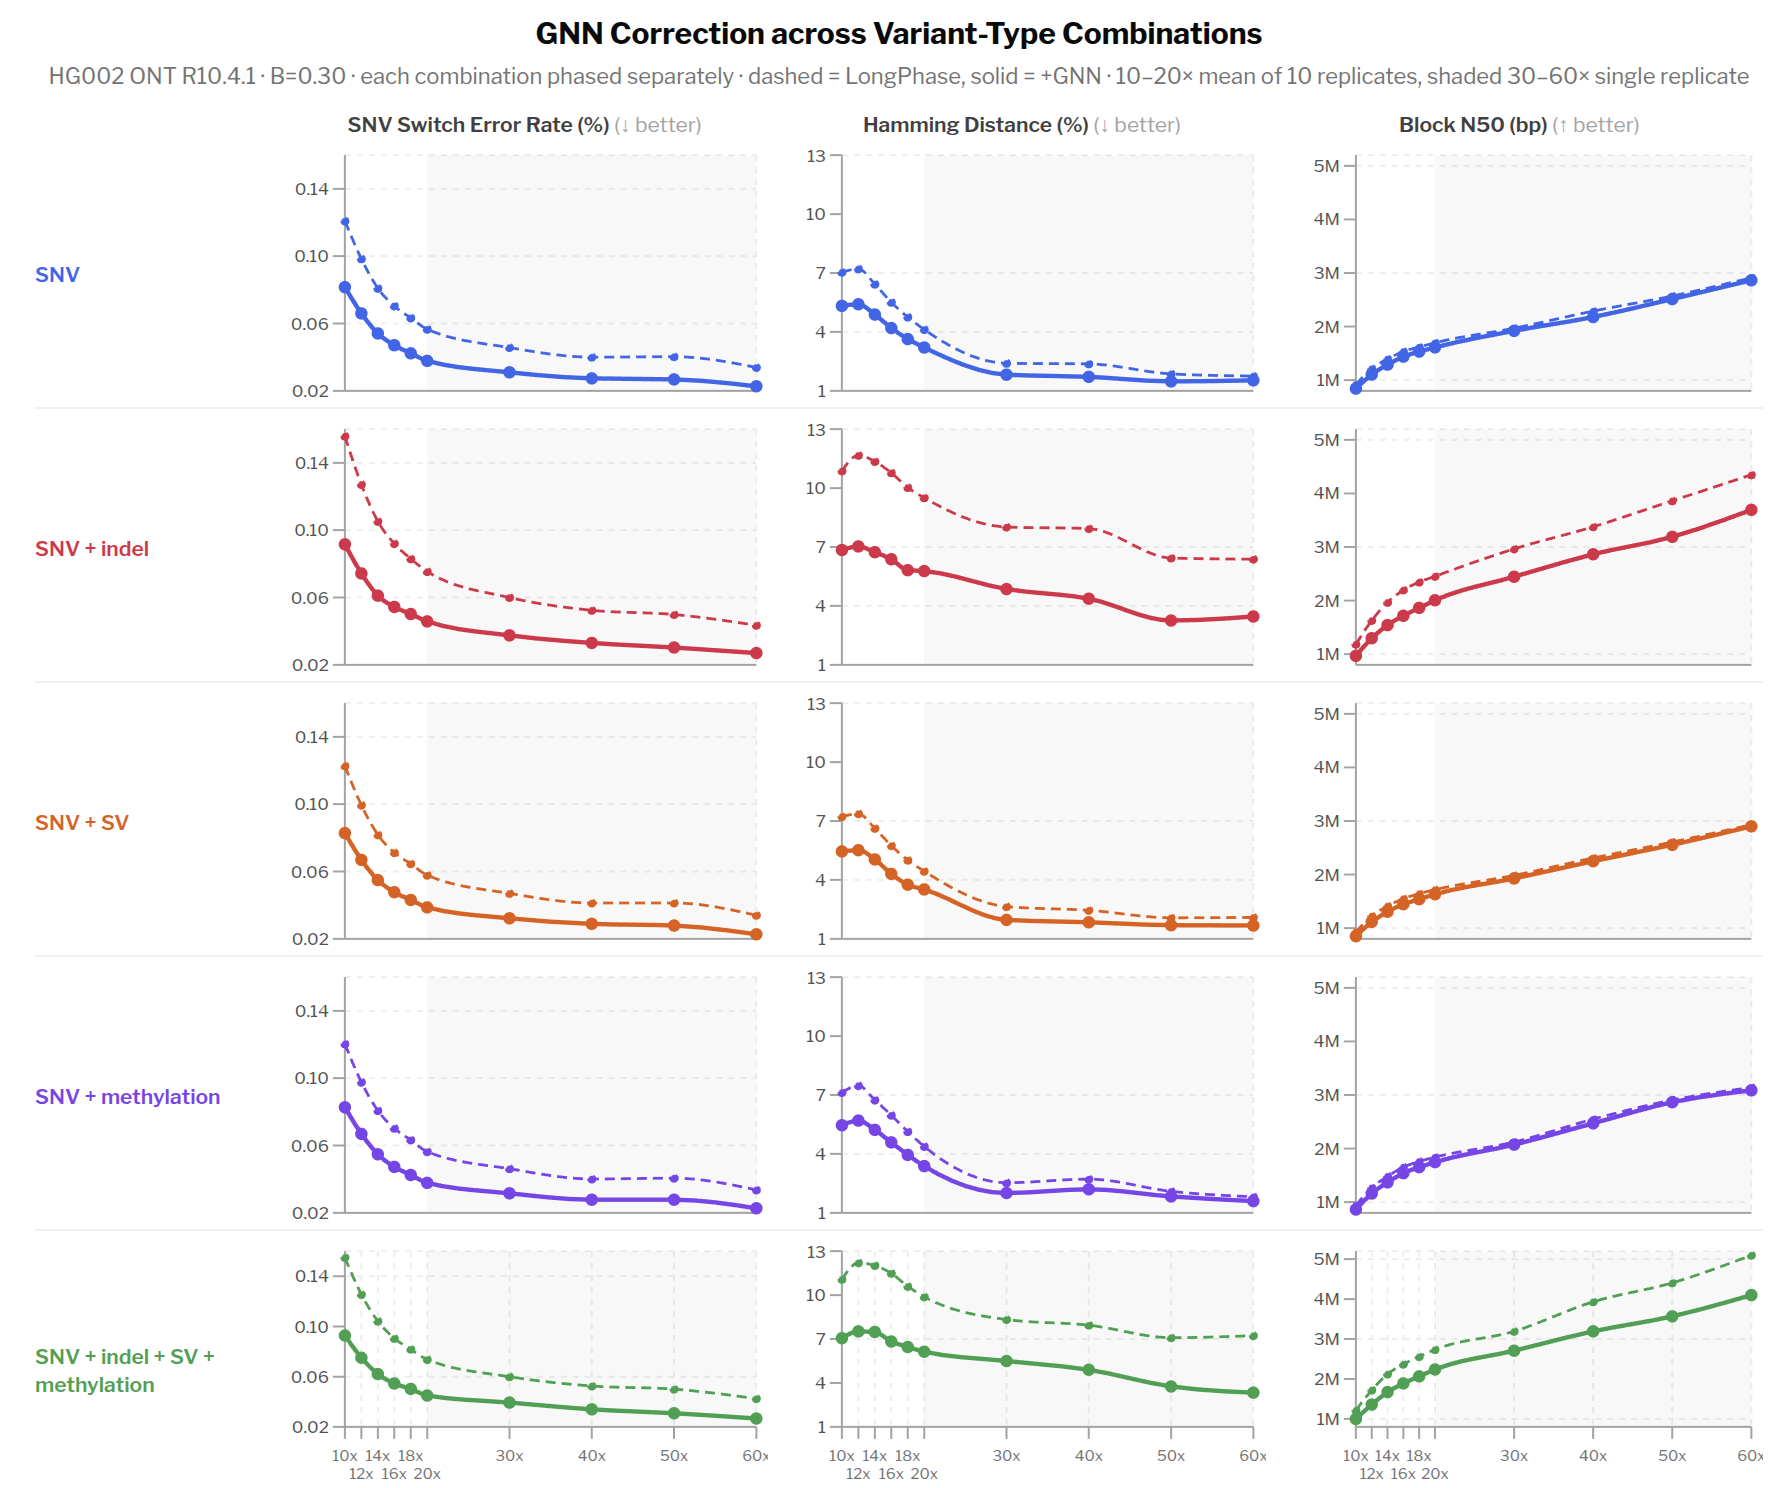
\includegraphics[width=0.92\textwidth]{fig5_variant_combinations}
  \caption{\textbf{Effect of neural-network correction across variant-class combinations.}
  Each row is a separate phasing run of HG002 nanopore R10.4.1 data with the indicated variant classes; dashed, \toolname; solid, \toolname with correction. Columns: SNV switch error rate, Hamming distance and phase-block N50, scored against the v5.0q benchmark on SNVs. Replicates as in Fig.~\ref{fig:snv}.}
  \label{fig:combinations}
\end{figure}

\begin{figure}[p]
  \centering
  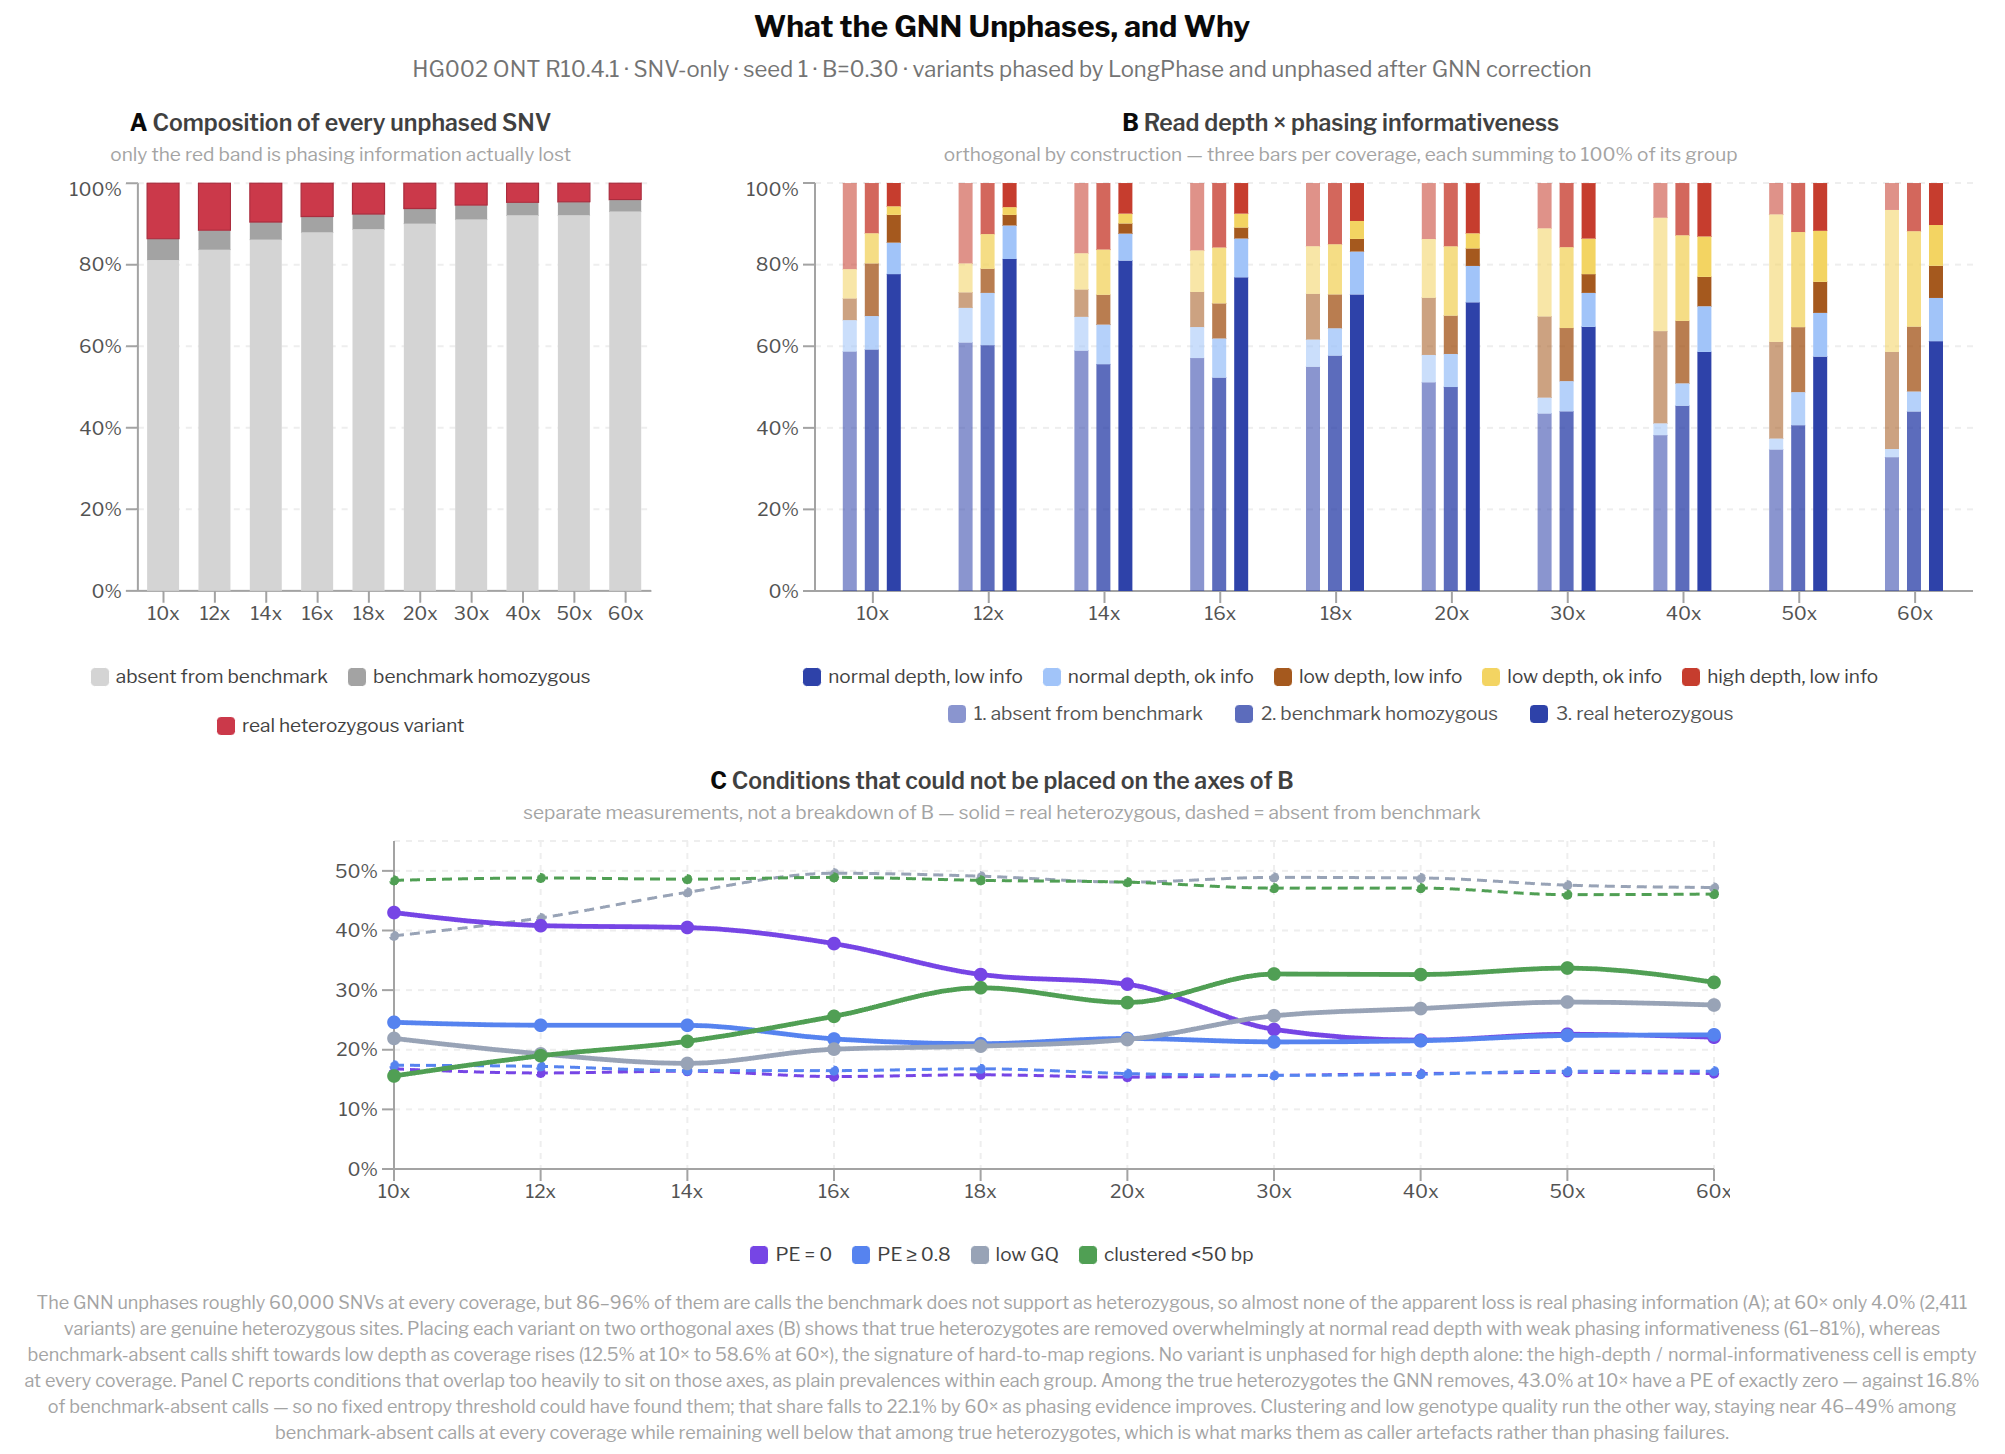
\includegraphics[width=\textwidth]{fig6_unphased_analysis}
  \caption{\textbf{Composition of the variants unphased by the neural network.}
  SNV-only phasing of HG002 nanopore R10.4.1 data (one down-sampling replicate, seed 1; break threshold 0.30); every SNV phased by \toolname and unphased after correction ($\sim$60,000 per coverage) is classified against the v5.0q benchmark.
  \textbf{a}, Fraction of unphased SNVs that are absent from the benchmark, homozygous in the benchmark or genuine heterozygous sites; only the last category represents lost phasing information.
  \textbf{b}, Within each of the three categories, distribution over read depth (low, normal, high relative to the genome-wide mean) and phasing informativeness (number of informative linking reads); the three bars at each coverage each sum to 100\% of their category.
  \textbf{c}, Prevalence of conditions that overlap the axes of \textbf{b}: phasing entropy of exactly 0, phasing entropy $\ge 0.8$, low genotype quality and clustering within 50~bp of another variant; solid, genuine heterozygous sites; dashed, benchmark-absent calls.}
  \label{fig:unphased}
\end{figure}


\section*{Discussion}
% ------------------------------------------------------------------
%  Discussion (no subheadings, ~1,200 words;
%  interpretation, relation to prior work, limitations, outlook).
%  \todo{If the editor enforces a hard 1,000-word Discussion, the two
%  cheapest cuts are (i) the alternative-route sentence opening the
%  final paragraph (trio/Hi-C/Strand-seq/imputation, ~55 words) and
%  (ii) the assembly-graph-GNN analogy in paragraph 3 (~20 words);
%  neither carries a claim made nowhere else.}
% ------------------------------------------------------------------

\toolname brings together two ideas that read-based phasing has so far kept apart. The first is that every class of heterozygous evidence a read carries belongs in one haplotype model; the second is that a phaser should report, variant by variant, how far its output can be trusted. The first extends an observation made independently for methylation\cite{akbari2021nanomethphase,fu2024methphaser,akbari2023parentoforigin} and for SVs\cite{lin2022longphase,holt2024hiphase}, namely that SNVs alone leave haplotype blocks stranded wherever heterozygosity is low. Calling allele-specific 5mC from modification tags into the same weighted graph as SNVs, indels and SVs raises block N50 above SNV-only phasing by more than 70\% at 60$\times$ (5.0 versus 2.9~Mb; 40\% after correction), with no post-processing step and on nanopore rather than HiFi reads, to which joint small- and structural-variant phasing had been confined\cite{holt2024hiphase}. The second idea gives downstream analyses a measure of phase reliability comparable to the genotype quality attached to variant calls, and to the posteriors that statistical phasers have long reported for imputed haplotypes\cite{hofmeister2023shapeit5}. That measure replaces the binary phased-or-unphased state that read-based tools, ours included, have reported until now.

Perhaps the most consequential finding here concerns evaluation rather than algorithms. Scored against two truth sets, the same phased VCFs on the same reference give different error magnitudes and, for some tools, a different ordering. GIAB v4.2.1\cite{wagner2022giab} excludes most segmental duplications, satellite arrays and large tandem repeats from assessment\cite{olson2023benchmarking,dwarshuis2024stratifications}; the benchmark derived from the complete diploid T2T-HG002 assembly\cite{hansen2026q100,jarvis2022hg002}, projected onto GRCh38, adds some 700~Mb of autosomal sequence that v4.2.1 never assessed, most of it satellite and segmentally duplicated\cite{hansen2026q100}. Every tool accumulates more switch errors under the T2T-based benchmark, in rate as in absolute terms, and the spread between tools widens from under 30\% to three- to fivefold. That widening is what one would expect if mis-mapped reads, homopolymer errors and collapsed paralogues create systematically wrong linkages rather than random noise, which is what the evidence calibration in \toolname targets; we have not stratified switch errors by genomic context to test that directly. The ranking can also invert. \longphase~1.0 made more switch errors than \whatshap under v4.2.1 and fewer under the T2T-based benchmark. Almost every published comparison of phasers\cite{patterson2015whatshap,edge2017hapcut2,shafin2021margin,holt2024hiphase,fu2024methphaser,lin2022longphase} used GRCh38-based GIAB releases and so describes the easier part of the genome, much as variant-calling benchmarks did before complete references exposed the rest\cite{aganezov2022complete,olson2023benchmarking}. Two observations suggest that the extra errors are genuine and not artefacts of a draft truth set. Hamming distance is nearly unchanged between benchmarks for the four current tools, which points to isolated switches and not to the long-range disagreements a mis-projected benchmark would create. The advantage of \toolname over \whatshap and \hapcut also persists under v4.2.1, though with a smaller margin. The T2T-HG002 benchmark is nonetheless still being refined, and residual discordance in the hardest regions may be benchmark rather than phasing error; comparisons should therefore report both truth sets and stratify switch errors by genomic context\cite{dwarshuis2024stratifications,nurk2022t2t,liao2023pangenome}.

The neural network was designed to complement the graph algorithm, not to replace it. Where Ralphi\cite{battistella2025ralphi} and GCphase\cite{luo2024gcphase} learn haplotype assembly itself and must scale to whole chromosomes, \toolname confines learning to windows around high-entropy variants; inference costs one to two minutes per genome and fewer than 700,000 parameters compile into the binary. The closest precedent is the likelihood-based pruning of \hapcut\cite{edge2017hapcut2}, which withholds variants whose posterior under the phasing model falls below a threshold. Our correction conditions on something else. In place of the likelihood that produced the phase, a model that treats reads as independent and correctly placed, the network reads the structure of the evidence across a window: vote totals, entropy, sequence context, graph topology and the concordance of neighbours. That is where correlated errors from mis-mapped reads and paralogues leave a trace. Because the correction only withholds phase, one might object that fewer switch errors simply reflect a smaller denominator. Three observations speak against that reading. The rate is computed per assessed pair, and of the roughly 60,000 SNVs unphased at 60$\times$ only 2,411 are heterozygous in the benchmark and enter that denominator, far too few to explain the fall from 740 to 490 genome-wide switch errors. Block N50 is almost unaffected (2.87 versus 2.9~Mb), which pruning informative links could not achieve. And the phased fraction stays within about a percentage point of \whatshap (91.6\% versus 92.5\% at 30--60$\times$)\todo{confirm 91.6\% is the phased fraction after correction; this argument rests on it}. At 10$\times$ the trade is less favourable, with 14\% of what is unphased being genuine heterozygotes and N50 falling from 0.93 to 0.84~Mb. Even there the trade remains worth making, because 86--96\% of what is removed are calls the benchmark does not support as heterozygous, mostly caller artefacts at clustered or low-quality sites whose spurious phase would otherwise reach haplotagged reads and the somatic callers that consume those reads\cite{zheng2026clairs,chen2025clairsto,keskus2025severus}.

Several limitations remain. The network was trained and evaluated on one individual, HG002, sequenced on a single nanopore chemistry\todo{Methods must state which HG002 chromosomes and coverages were held out of training, and which truth set supplied the training labels; without a chromosome-level hold-out the evaluation is circular}. Two choices bound the overfitting: the features are generic (vote counts, entropy, sequence context, graph topology; no sequence embeddings, no sample-specific statistics), and the output is restricted to withholding phase, so a miscalibrated model costs contiguity and cannot invent haplotypes. Transfer to PacBio HiFi, duplex chemistry and non-human genomes is untested; the graph algorithm supports both platforms, but for the network reported here cross-platform performance is an expectation, not a result. Indel co-phasing is a trade-off we have accepted rather than solved. Adding indels lengthens blocks but raises the uncorrected SNV switch error rate (0.035\% to 0.048\% at 60$\times$), and is worth taking only because correction more than repays the loss, leaving four-class co-phasing both more accurate and 40\% longer-blocked than uncorrected SNV-only phasing. Better indel calling\cite{zheng2026accelerated,kolesnikov2024local} would remove the trade-off altogether, and SNV-only phasing remains available in the meantime. The phased fraction of SVs and indels is bounded by the upstream callers, and 5mC co-phasing requires modification-aware base calling, whose accuracy varies between callers and chemistries\cite{sigurpalsdottir2024methylation}, and \texttt{MM}/\texttt{ML} tags retained through alignment. Finally, \toolname assumes a diploid genome with balanced allele fractions.

Trio assembly\cite{cheng2021hifiasm,rautiainen2023verkko}, Hi-C\cite{selvaraj2013hic} and Strand-seq\cite{porubsky2021fully} reach chromosome scale but need extra samples or libraries, and imputation\cite{sun2025advances,ebler2022pangenie} depends on panels still sparse for structural variation and many populations; \toolname needs one sample and one library, and per-variant phase reliability makes the resulting haplotypes a natural input to hybrid read-plus-panel strategies\cite{liao2023pangenome,hofmeister2023shapeit5}. As a drop-in replacement in pipelines already built on \longphase\cite{zheng2022clair3,zheng2026clairs,keskus2025severus,ont2025wfhuman}, \toolname delivers the new annotations without interface changes, and those annotations have concrete uses. A compound-heterozygous diagnosis rests on a single \textit{trans} call between two variants in one gene\cite{eisfeldt2025clinical,negi2025napu}; the entropy of those variants and of the links between them turns that call into a quantity a diagnostic report can qualify, flagging the cases that warrant a confirmatory assay. Allele-specific methylation analyses currently treat every haplotagged read alike, whereas weighting reads by the confidence of the variants that tagged them would keep imprinting and \textit{cis}-regulatory signals\cite{akbari2023parentoforigin} from being diluted by thinly supported blocks. Haplotype-aware somatic callers\cite{zheng2026clairs,keskus2025severus} likewise accept inherited phase without qualification, and propagating entropy would let them discount the loci at which switch errors concentrate. Realising any of this will require downstream tools to read the new fields, much as they came to read genotype quality.


\section*{Methods}
% ------------------------------------------------------------------
%  Methods (bold run-in subheadings, past tense,
%  enough detail to reproduce).
%
%  PROVENANCE OF EVERY ALGORITHMIC STATEMENT BELOW:
%  verified line-by-line against the JH branch of
%  github.com/twolinin/longphase, commit cc17fb1 ("Remove ONNX",
%  2026-08-25), which is both the tip of JH as of 2026-09-18 (re-checked
%  after `git fetch`) and the state of the code that produced the
%  results reported here. Where the text and that commit disagreed, the disagreement is
%  marked with a \todo{} that names the file and line checked, rather
%  than being silently rewritten. Note that the checked-out `main`
%  branch (v2.0.2, commit 79abbb3) does NOT contain Compare.cpp,
%  GNN*.cpp/.h or GNNWeights.h; the gnn and compare sub-commands exist
%  only on JH. \todo{Merge JH into main and cut a release before
%  submission, then replace every "JH/cc17fb1" reference here and in
%  the Supplementary with the release tag; reviewers must be able to
%  obtain the exact binary.}
%
%  Supplementary cross-references in this file are HARD-CODED numbers,
%  not \ref keys, because main.tex and Supplementary.tex are separate
%  documents. All nine Supplementary Figures (2026-09-19: former Figs. 2+3,
%  1+4 and 7+9 merged; the rest renumbered) and all six Supplementary
%  Tables (2026-09-20: parameter tables removed) cited below were checked to exist and to point at the intended
%  item on 2026-09-19. Re-check after any reordering of
%  Supplementary.tex.
% ------------------------------------------------------------------

\subsection*{Overview of \toolname}
\toolname takes as input long-read alignments (BAM or CRAM), a reference genome and heterozygous variant calls, and produces phased VCF files for every variant class together with haplotagged alignments (Fig.~\ref{fig:overview}). The pipeline comprises four sub-commands implemented in a single C++ binary linked against HTSlib\cite{bonfield2021htslib}: \texttt{modcall} identifies allele-specific 5-methylcytosine (5mC) sites from the \texttt{MM}/\texttt{ML} modification tags of the alignments; \texttt{phase} co-phases SNVs, small indels, SVs and 5mC sites in one weighted phasing graph per chromosome and emits per-variant phasing diagnostics; the optional \texttt{gnn} sub-command applies a graph neural network to the diagnostics and removes phase assignments that are predicted to be erroneous; and \texttt{haplotag} assigns each read to a haplotype using the phased variants. A fifth sub-command, \texttt{compare}, implements the evaluation metrics (below). \texttt{phase}, \texttt{modcall} and \texttt{compare} are parallelized over chromosomes with OpenMP; \texttt{gnn} distributes trigger windows over a pool of C++ threads, sharing one immutable copy of the network weights. The graph phasing algorithm extends the design of \longphase~1\cite{lin2022longphase}; the sections below describe the current algorithm, with the implementation-level detail of the individual modules in Supplementary Methods~1--6; command-line parameters and their defaults are documented in the repository (Code availability). \toolname is a germline, diploid phaser.

\subsection*{Input variant calls}
Heterozygous SNVs and small indels were taken from a standard long-read small-variant caller (Clair3\cite{zheng2022clair3} in this study); homozygous and filtered records are carried through to the output unchanged but do not enter the graph. With \texttt{--indels}, small indels were phased alongside SNVs; indels with \texttt{QUAL} below a user threshold (\texttt{--indelQuality}, default 0, i.e.\ disabled) were excluded and marked in the output \texttt{FILTER} column. Each indel was additionally annotated as lying in a tandem repeat, because indel calls in repetitive sequence are the class most often misplaced by the caller and, once misplaced, link the wrong alleles. The dinucleotide immediately 3$'$ of the indel position was read from the reference, and the indel was flagged when that dinucleotide recurred in five consecutive copies. Only dinucleotide units are considered; extending the test to trinucleotide units was evaluated during development, did not reduce switch errors consistently across coverages and was therefore not adopted. Flagged indels were not discarded but retained as phasing evidence, casting votes at one-tenth weight (see below), so that they can still bridge SNV-poor regions without dominating a contested decision. SVs were taken from Sniffles2\cite{smolka2024sniffles2} or cuteSV\cite{jiang2020cutesv} run with read-name reporting (\texttt{--output-rnames} or \texttt{--report\_readid}); homozygous SVs, SVs whose breakpoint coincides with an SNV, and SVs with duplicated positions were excluded. For each retained SV we recorded the set of supporting read names and the SV length.

\subsection*{Calling allele-specific methylation (\texttt{modcall})}
Base-level modification probabilities (Supplementary Fig.~7) were read from the \texttt{MM}/\texttt{ML} tags produced by Dorado\cite{ont2025dorado} and carried into the alignments by \texttt{minimap2 -y}\cite{li2018minimap2}; PacBio HiFi reads carry the same tags but were not used in this study. For each CpG on each read, the base was labelled methylated if the 5mC probability was $\ge 0.8$ (\texttt{--modThreshold}) and unmethylated if that probability was $\le 0.2$ (\texttt{--unModThreshold}); intermediate values were treated as noise. Only the 5mC probability (modification code \texttt{m}) was read (\texttt{ModCallParsingBam.cpp}:169). 5hmC calls (code \texttt{h}) were ignored, so under a 5mCG\_5hmCG basecalling model a cytosine called as 5hmC was counted as unmethylated whenever its 5mC probability was $\le 0.2$. Reads on the reverse strand were mapped to the forward-strand CpG coordinate and the two strands of each CpG were genotyped jointly. Each read was thereby assigned to one of three states at the site, and a site was called heterozygous (allele-specifically methylated) when the two states were balanced and the ambiguous fraction small:
\begin{equation}
\frac{\min(M_R,U_R)}{\max(M_R,U_R)} \ge 0.6 \;\;(\texttt{--heterRatio}),
\qquad
\frac{A_R}{M_R+U_R+A_R} \le 0.2 \;\;(\texttt{--noiseRatio}),
\label{eq:hetmeth}
\end{equation}
where $M_R$, $U_R$ and $A_R$ are the numbers of methylated, unmethylated and ambiguous reads; otherwise the site was called homozygous methylated or unmethylated and excluded from phasing. Only CpG dinucleotides were considered; modification calls at non-CpG cytosines were discarded.

A site passing equation~(\ref{eq:hetmeth}) is balanced but not necessarily allele-specific, because a site at which methylation varies stochastically between reads satisfies the same inequalities. Candidate sites were therefore required to co-segregate with a neighbouring heterozygous marker. Writing $RR$, $RA$, $AR$ and $AA$ for the numbers of reads carrying each of the four combinations of the two states at a pair of sites, a pair was accepted as linked when
\begin{equation}
\frac{\max(RR+AA,\; RA+AR)}{RR+AA+RA+AR} \ge 0.9 \;\;(\texttt{--connectConfidence}),
\label{eq:linkmeth}
\end{equation}
that is, when nearly every read supports one of the two possible pairings rather than a mixture. Equation~(\ref{eq:linkmeth}) is the criterion the phasing graph itself applies to a pair of alleles, so the two methylation states enter the graph on the same footing as reference and alternate alleles and \texttt{phase} requires no methylation-specific machinery.

Linking was applied in two modes: \emph{SNV-anchored}, used whenever an SNV VCF was supplied, in which a candidate CpG must satisfy equation~(\ref{eq:linkmeth}) against an SNV among the next 20 variants (\texttt{--connectAdjacent}); and \emph{methylation-only}, used where no informative SNV is in range, in which the same criterion is applied between two candidate CpGs. Candidates that never satisfied it were held back as weak points and admitted only on a later pass against an already accepted CpG. Runs of consecutive CpG coordinates were then merged into a single locus represented by the first position, which consolidates the forward- and reverse-strand calls of a run into one read list and removes the need for \texttt{phase} to reason about strand. The resulting VCF records the methylated and unmethylated read names (\texttt{MR}, \texttt{NR}), the read strand and the per-site depths, and is passed to \texttt{phase} through \texttt{--mod-file}. The depth bound on the neighbour scan, the weak-point expansion and the rationale for merging are given in Supplementary Method 1. The values quoted here are the compiled-in defaults.

\subsection*{Extraction of read-level allele observations}
For each chromosome, all alignments with mapping quality $\ge 1$ (\texttt{--mappingQuality}) that were not unmapped, secondary or marked as optical/PCR duplicates were streamed once and, for every variant they overlap, converted into an allele observation with an associated quality. Supplementary alignments were retained as phasing evidence, which is why the overlapping-alignment filter below is required; this differs from the stricter filters applied inside \texttt{modcall} and \texttt{haplotag}. SNV alleles were read from the aligned base and inherited its Phred base quality; indel alleles were called from the CIGAR string; SV alleles were assigned by scanning a window of 20 CIGAR operations (\texttt{--svWindow}) around the SV start for an insertion or deletion whose length is within 10\% of the SV length (\texttt{--svThreshold}), and reads named by the SV caller were also assigned the ALT allele; and 5mC alleles were taken from the \texttt{modcall} read lists. Soft- and hard-clipping operations longer than 5~bp were counted per reference position, separately for clips at the front (left) and back (right) end of an alignment, as evidence of alignment breakpoints for copy-number detection (below). Supplementary Method 2 gives the per-class extraction rules in full. 


Three filters were applied before graph construction. (1)~\textit{Homopolymer SNV filter}, applied under \texttt{--ont} only: when two SNVs both lie in homopolymers of length $\ge 3$ and are $\le 2$~bp apart, the downstream SNV was removed, because such pairs are dominated by systematic homopolymer-length errors in nanopore reads. (2)~\textit{Overlapping-alignment filter}: when two alignments of the same read overlapped by more than 20\% of their combined span (\texttt{--overlapThreshold}), the shorter alignment was discarded. (3)~\textit{Copy-number-aware filter} (Supplementary Fig.~1e,f). Collapsed paralogues and copy-number-altered segments recruit reads from more than one locus, so that paralogue-specific differences are called as heterozygous variants and link alleles that are not on the same chromosome. Such segments are bounded by alignment breakpoints. Two boundary shapes were detected from the per-position front- and back-clip counts by a three-state scanner: a \emph{step} boundary, characteristic of a copy-number transition, declared on a cluster of at least five front-clips at one position, and a \emph{ramp} boundary, characteristic of the progressively nested breakpoints left by breakage--fusion--bridge cycles, declared where front-clips merely exceed back-clips. Both active states carried a running excess of front- over back-clips, extended the candidate interval by a 30~kb look-ahead while that excess was large, and closed on a back-clip threshold scaled to the strength of the breakpoint that opened the interval; candidates longer than 200~kb, or in which the excess fell to zero, were abandoned. Supplementary Method 2 gives the state machine, its five constants and the closing rules in full.

%  [optional figure] The 0.7 threshold in equation~(\ref{eq:cnvmr}) is presented
%  here without evidence, but the evidence exists: the TP/FP histogram of
%  $\mathrm{MR}(v)$ on HG002 (true heterozygous sites concentrated below 0.7,
%  false calls piled at 0.8--1.0) is already in the group's algorithm slides and
%  should be added as Supplementary Fig.~1g with the threshold marked. Regenerate
%  it with the submitted version on the Clair3 calls and coverages used in this
%  paper: the slide version used DeepVariant v1.9.0 calls and a pre-release
%  1.7.3-era build, so the distribution shown there does not describe the filter
%  as it now stands. The interval and removal counts a reviewer will ask for are
%  listed in the \texttt{todo} of Supplementary Method 2.
Within each interval, every read was scored by its \emph{mismatch load} $R_m$, the number of heterozygous sites inside the interval at which the read carries the alternate allele, and every heterozygous variant $v$ in the interval was then scored by
\begin{equation}
\mathrm{MR}(v) = \frac{\bar{R}_m^{\,\mathrm{ALT}}}{\bar{R}_m^{\,\mathrm{REF}} + \bar{R}_m^{\,\mathrm{ALT}}},
\label{eq:cnvmr}
\end{equation}
where $\bar{R}_m^{\,\mathrm{ALT}}$ and $\bar{R}_m^{\,\mathrm{REF}}$ are the mean loads over the reads supporting the alternate and the reference allele of $v$. Variants with $\mathrm{MR}(v) \ge 0.7$ were removed from all reads; Supplementary Method 2 explains why the statistic separates genuine heterozygous sites from paralogue-specific differences. 

\subsection*{Weighted phasing graph}
Each heterozygous variant $v$ contributes two nodes (Supplementary Figs.~1--2), $v^{\mathrm{ref}}$ and $v^{\mathrm{alt}}$. For every read, the observed alleles were sorted by position and each allele node was connected to the allele nodes of the next $k = 35$ variants on the same read (\texttt{--connectAdjacent}); no distance limit is applied to these edges or to the votes cast along them, so a single read can link variants more than 300~kb apart. The \texttt{--distance} parameter (300~kb) acts instead on the variant sequence: a variant whose next heterozygous variant lies further away than this is skipped during haplotype resolution, casting no votes and receiving no haplotype or entropy, so that a block cannot be carried across a gap in heterozygosity. Each read contributes a weight of 1 to the edge if both of the two observations have Phred quality $\ge 12$ (\texttt{--baseQuality}) and a weight of 0.1 (\texttt{--edgeWeight}) otherwise. Observations without a base quality were assigned a fixed one (\texttt{PhasingGraph.cpp}:838--862): 60 for indel and 5mC observations and for SV observations carrying the ALT allele, and 30 for SV observations on reads that neither the CIGAR scan nor the caller's read list assigned to the ALT allele, which are taken to carry the reference allele. Both values exceed the default base-quality threshold, so at default settings every indel, SV and 5mC observation contributes a weight of 1; the lower quality of reference-allele SV observations reduces their weight only when \texttt{--baseQuality} exceeds 30. For a pair of variants $(u,v)$ this yields four accumulated weights $w_{rr}, w_{ra}, w_{ar}, w_{aa}$, the total support for the two allele pairings $P = w_{rr}+w_{aa}$ (\textit{cis} between reference alleles) and $Q = w_{ra}+w_{ar}$, and their similarity $s = \min(P,Q)/\max(P,Q)$.

\subsection*{Haplotype resolution by multi-neighbour voting}
Variants were processed in coordinate order. For the current variant $u$, each of its $k$ downstream neighbours $v$ received a vote for the pairing with the larger support ($P$ versus $Q$). A pair was declared uninformative and cast no vote if $s > 0.7$ (\texttt{--edgeThreshold}); for SNV--5mC pairs the threshold was 0.3, and such pairs cast no vote at all when their total accumulated support was below 1. Votes were weighted: 1 by default; 20 when the pairing was near-unanimous ($s \le 0.1$ with total support $\ge 1$, or one pairing accumulated less than 1 unit of support while the other accumulated at least 1); and 0.1 when the voting variant was a tandem-repeat indel. \todo{The weight-20 branch in \texttt{PhasingGraph.cpp} was chained off \texttt{if(debug)} at cc17fb1; the fix is applied in the working tree of the source repository (uncommitted as of 2026-09-20) and must be committed before the release. \texttt{findBestEdgePair} still takes an unused \texttt{isONT} argument.} The vote was translated into a haplotype vote for $v$ using the already assigned haplotype of $u$, and the two weighted haplotype totals $h_1(v)$ and $h_2(v)$ were accumulated from all upstream voters. A guard against a single erroneous ultra-long read counted, among the votes received by $v$, those whose total support was at most 1 read-equivalent; when more than three such votes existed and at least one qualifying vote remained, $h_1$ and $h_2$ were recomputed from only those votes with $s < 0.2$, weight $\ge 1$ and a voting variant that is not a small indel. Variant $v$ was assigned to the haplotype with the larger total. When $h_1 = h_2$ (including the case of no votes at all) and $v$ lay beyond the last position reached by any accepted edge, a new phase block was opened at $v$; a tie at a position already covered by an accepted edge left the previous block intact and the tied variant unphased, casting no votes. Blocks were identified by the position of their first variant, which defines the \texttt{PS} tag. The six constants of this rule were fixed by a sweep on HG002 at 10--60$\times$ before the experiments reported here and were not re-tuned afterwards; Supplementary Method 3 states them and Supplementary Fig.~9 shows the sweeps.



\subsection*{Read-based correction}
After the initial assignment (Supplementary Fig.~3), every read was assigned to a haplotype by weighted majority over its phased alleles, with SNV and SV alleles contributing 1, indel and tandem-repeat-indel alleles 0.1, and 5mC alleles nothing; a read was tagged only if the majority fraction exceeded 0.65 (\texttt{--readConfidence}) and the total weighted evidence exceeded 1. The allele counts of the two read populations were then used to re-derive each variant's phase: the fraction of tagged reads consistent with the assignment $\rho = \max(n_1, n_2)/(n_1+n_2)$, where $n_1$ and $n_2$ count haplotype-1 reads carrying the reference allele plus haplotype-2 reads carrying the alternate allele and vice versa, had to exceed 0.75 (\texttt{--snpConfidence}); otherwise the variant was left unphased. This second pass removes assignments driven by a small number of chimeric or mis-mapped reads.

\subsection*{Phasing entropy and graph export}
For each phased variant we recorded the two weighted haplotype totals $h_1$ and $h_2$ (after the single-read guard, where that guard fired) and their normalized Shannon entropy
\begin{equation}
\mathrm{PE}(v) = -\sum_{i \in \{1,2\}} p_i \log_2 p_i, \qquad p_i = \frac{h_i}{h_1+h_2},
\end{equation}
which ranges from 0 (unanimous votes) to 1~bit (equal support for both haplotypes), with the convention $0\log_2 0 = 0$. $\mathrm{PE}$ is set to 0 when $h_1+h_2=0$, so a value of exactly 0 denotes either unanimous support or no votes at all; the two cases are distinguished by \texttt{H1}$+$\texttt{H2}, and the second arises only at the first variant of a phase block, the one position at which a variant without votes is phased (Supplementary Fig.~2f). $\mathrm{PE}$, $h_1$ and $h_2$ are written to the output VCF as the \texttt{INFO} fields \texttt{PE}, \texttt{H1} and \texttt{H2}. With \texttt{--dot}, the per-chromosome phasing graph is written in DOT format as \texttt{<prefix>.<chrom>.dot}, one directed edge $u^{a}\rightarrow v^{b}$ per accepted voting pair with the haplotype weight accumulated at $u$ at the time the vote was cast as label; these files are the input of the GNN module.

\subsection*{Graph neural network for phase-error detection}
The graph neural network (GNN) operates on local windows of the phasing graph and predicts, for each variant, the probability that its phase assignment is wrong (Supplementary Figs.~4--6). Only records that are heterozygous and phased in the input VCFs enter the module. Variant records from the SNV/indel, SV and 5mC VCFs were merged and sorted by position so that windows span all co-phased variant classes, and a window was opened around every such variant with $\mathrm{PE} \ge 0.8$ (\texttt{--pe-threshold}), extending 20 variants (\texttt{--window}) on each side of the trigger in that merged list. A window therefore contains at most $2\times 20 + 1 = 41$ variants and $82$ allele nodes. Windows with more than 256 nodes are skipped; at the default window size this cap is never reached, and binds only for \texttt{--window} greater than 63.

\textit{Node and edge features.} Each allele node carries 31 features in four groups: phasing evidence ($\mathrm{PE}$, the genotype and allele indices, the trigger and phase-set indicators, the signed offset from the trigger normalized by the largest absolute offset in the window, the two weighted haplotype totals $h_1$ and $h_2$, and six transforms of them); genomic context, computed from the reference when \texttt{-r} is given and zero otherwise (homopolymer length, GC content, tandem-repeat unit count, local sequence entropy, variant density and distance to the nearest indel); graph structure (out-degree, phase-set size, log offset from the trigger, dispersion of the outgoing edge weights and a bridge-vertex indicator); and four one-hot variant-class indicators. Each edge carries six features derived from the DOT vote weight $w$, the genomic distance, the allele-index match and the phase-set relation. Edges are restricted to pairs with both endpoints inside the window, symmetrized, and augmented with one self-loop per node whose features are the mean of its non-self incident edges. Supplementary Tables~1 and~2 give every feature with its exact definition, normalization and cap, and Supplementary Method 4 gives the transforms and the provenance of $h_1$ and $h_2$.

\textit{Architecture.} The network follows the general, powerful, scalable (GPS) graph-transformer recipe\cite{rampasek2022gps}. Node features were standardized by a batch-normalization layer whose statistics are frozen at inference, projected linearly to a 128-dimensional embedding and passed through a GELU non-linearity. Four identical layers follow, each combining a local branch, a four-head GATv2 message-passing layer over the window's edges\cite{velickovic2018gat,brody2022gatv2}, with a global branch, four-head scaled dot-product self-attention over all nodes of the window\cite{vaswani2017attention}. The two branch outputs are added to the residual stream and layer-normalized, then passed through a two-layer feed-forward block (128$\rightarrow$256$\rightarrow$128, GELU) with a second residual connection and layer normalization. The final node embedding is concatenated with two edge-context scalars and passed through a two-layer classifier (130$\rightarrow$128$\rightarrow$2) with softmax output.

The model comprises 687,358 float32 values (2,749,432~bytes). Inference is implemented in plain C++ with dense $N\times N$ adjacency and edge tensors and no external runtime dependencies. Predictions for the two allele nodes of a variant were averaged, and a variant covered by several windows received the running mean of its predictions. Only variants in the central zone of a window were scored, namely those no further from the trigger than half the window's largest trigger distance; this is the same zone the network was trained to score, and nodes outside it are read as context but never scored. The attention equations, the edge-context definition, the requirement for the exact erf-based GELU and the central-zone rule are given in Supplementary Method 4; the hyperparameters are in Supplementary Table~3.

\textit{Training data.} Training windows were produced from \toolname co-phasing runs on the same HG002 ONT R10.4.1 alignments that the evaluation uses, at the six coverages 10, 12, 14, 16, 18 and 20$\times$ and at all ten down-sampling replicates of each, that is from 60 phasing runs. Each run contributed its SNV/indel, SV and 5mC VCFs together with the per-chromosome DOT export, and windows were opened by the same rules as at inference (\texttt{--pe\_threshold 0.8}, \texttt{--window 20}); the genomic-context features were computed from the same GRCh38 no-alt analysis set. Every window lies within a single chromosome, so the resulting 722,116 windows could be split by chromosome without any window straddling a boundary: chr1--chr14 and chr18--chr20 for training (602,788 windows, 18,356,880 labelled allele nodes in the scored zone), chr15 and chr16 for validation (67,880 windows, 1,509,576 nodes) and chr17, chr21 and chr22 for testing (51,448 windows, 1,367,580 nodes). The training script verifies that the three chromosome sets are disjoint and aborts otherwise. All windows were drawn from the four-class co-phasing configuration, so SV and 5mC records enter the graphs the network was trained on, but only as context: the truth set used for labelling contains small variants alone, so no SV or 5mC node carried a label and among scored nodes only the SNV and indel indicators vary. At inference the module makes no such distinction: a variant's class enters only through the four indicator features, and SV and 5mC records are scored and unphased on the same footing as SNVs and indels. Corrections to SV and 5mC records are therefore unsupervised: they rest on transfer from the small variants that share their window, and their extent is reported in the Results (Fig.~\ref{fig:cophasing}c,d).





\textit{Labels.} Labels were derived from the v5.0q benchmark restricted to chr1--chr22 small variants, the same truth set used for evaluation, and describe the phase of a variant relative to its neighbours rather than in absolute terms. Within each window the variants were grouped by phase set, the first variant of a group present in the benchmark fixed that group's orientation, and later variants were labelled by whether their allele-to-haplotype orientation agreed with that anchor. Maximal runs of disagreement were then resolved so that a run is charged to the event that created it, not to each of its members: a single disagreeing variant was labelled \emph{unphase} if its $\mathrm{PE}$ was at least 0.9 and \emph{flip} otherwise, and in a run of two or more the first variant, the switch point, was labelled \emph{break} and the remaining members were reset to \emph{correct}. Variants absent from the benchmark, and all SV and 5mC records, were left unlabelled: they were masked from the loss but remained in the graph as context. The released model was trained in binary mode, in which \emph{flip}, \emph{unphase} and \emph{break} are merged into a single \emph{error} class, matching the single action the module is allowed to take. Supplementary Method 4 gives the labelling rules in full.

\textit{Class balance and loss.} Among the labelled central nodes of the training split, 17,812,710 (97.04\%) were \emph{correct} and 544,170 (2.96\%) \emph{error}, and 21.5\% of windows contained at least one error node. The imbalance was handled by subsampling, not by re-weighting the full distribution: each minibatch kept all of its error nodes and drew correct nodes uniformly at random to at most four times that number (\texttt{--ratio\_corr 4}), and because the draw was independent at every step the network saw the whole set of correct nodes over training. The cross-entropy on that subset was focal-weighted\cite{lin2017focal} by $(1-p_t)^{\gamma}$ with $\gamma = 1.5$ and used label smoothing of 0.05. Supplementary Method 4 explains why the error prevalence here is far above the genome-wide switch-error rate.

\textit{Training procedure.} Each window graph was made undirected before training by adding, for every DOT edge, a reverse edge carrying identical features; the DOT export is strictly one-directional (source position below target position), so without this a node could receive messages only from upstream, and read evidence is in any case symmetric. Two label-preserving augmentations, a haplotype swap and a coverage down-scaling, were applied to training windows only (Supplementary Method 4). Optimization used AdamW\cite{loshchilov2019adamw} with a peak learning rate of $3\times 10^{-4}$ and no warm-up, cosine annealing to $10^{-5}$ over a 100-epoch horizon, gradient-norm clipping at 1.0, and minibatches of 64 windows batched as disjoint graphs; the remaining optimizer settings are the PyTorch defaults and are listed with the rest of the training configuration in Supplementary Table~4. Dropout of 0.4 was applied to the output of the local branch, to the output of the global branch and inside each feed-forward block; dropout is inactive at inference and therefore does not appear in the exported graph. The run was seeded once (\texttt{--seed 42}, seeding both the Python and the PyTorch generators) and stopped early after 25 epochs without improvement of the validation criterion, at epoch 69 of the 100-epoch budget. Training used PyTorch 2.11.0 with PyTorch Geometric 2.7.0 under Python 3.12, CUDA 13.0 and cuDNN 9.19, on one NVIDIA GeForce RTX 5090. All reported \texttt{gnn} results come from this single training run; sensitivity to reseeding was not assessed.



\textit{Model selection.} Checkpoints were selected on the validation chromosomes by a net-gain criterion instead of validation loss or F1: at each epoch the predicted error probability was thresholded over 81 values spanning $[0.01,0.99]$ and the score $S = R\,(2 - 1/P)$ was maximized subject to a recall of at least 0.005, where $P$ and $R$ are the precision and recall of the error class. $S$ is the net fraction of true errors removed when a detection is worth one error and a false detection costs one, and is positive only for $P > 0.5$. The best checkpoint was epoch 44 ($S = 0.0235$, $P = 0.626$, $R = 0.058$, threshold 0.868). On the held-out chromosomes chr17, chr21 and chr22 it attained an accuracy of 0.941 with error-class precision, recall and F1 of 0.258, 0.499 and 0.340 under the argmax decision, over 41,378 labelled error nodes. The threshold applied by \texttt{gnn}, 0.30, is far more permissive, because the module's only action is to withhold phase: a false detection costs one phased variant rather than one switch error. Supplementary Method 4 gives the full selection procedure. \todo{State how 0.30 was chosen: a sweep, on which data and against which objective, or an a-priori choice. Add the phased-fraction/switch-error trade-off across thresholds as a supplementary panel.}

\textit{Export and numerical agreement.} The trained network was re-implemented with dense tensors, exported to ONNX and embedded in the binary as a base64-encoded float32 blob, and the forward pass refuses to run if the blob length disagrees with the expected parameter count. Numerical agreement was verified at each link of that chain; the largest observed difference in predicted error probability was $3\times 10^{-7}$, between the compiled C++ and ONNX Runtime on six synthetic graphs of 3--120 nodes. Supplementary Method 4 describes the export chain and the acceptance bounds.

%  [optional, cheap and recommended] Re-score at least one coverage restricted to
%  chr17, chr21 and chr22 (longphase compare --regions on the existing phased
%  VCFs) and report it beside the genome-wide value, so the gain can be read on
%  chromosomes that contributed no training window.
\textit{Hold-out design.} The hold-out is at the level of the chromosome. No window from chr17, chr21 or chr22 entered any gradient, any batch-normalization statistic or the checkpoint selection, and chr15 and chr16 were used only for selection. Nothing else was held out. The training windows come from the same 60 down-sampling replicates at 10--20$\times$ that Figs.~2--5 evaluate, the same v5.0q benchmark supplied both the training labels and the evaluation truth, and the figures are computed genome-wide over chr1--chr22, so 17 of the 22 evaluated chromosomes contributed training windows. No training window was drawn above 20$\times$, although results are reported to 60$\times$, and all training and evaluation data come from one individual (HG002) on one platform and chemistry. The consequences for generalization are discussed in the Discussion.

\textit{Correction.} A variant whose mean predicted error probability was $\ge 0.30$ (\texttt{--break-threshold}) was unphased: its genotype was rewritten in unordered, ascending form (\texttt{0|1} and \texttt{1|0} both become \texttt{0/1}) and its \texttt{PS} tag was removed, while the pair of alleles was preserved and no genotype was ever flipped. Bridge vertices may optionally be protected (\texttt{--respect-bridge}; off by default). After unphasing, the remaining phased variants of each phase set were checked for connectivity through the surviving DOT edges; when a phase set became disconnected, the largest component kept the original \texttt{PS} and every other component received a new \texttt{PS} equal to the 1-based position of its first variant (\texttt{--no-split-blocks} disables this). The corrected SNV/indel, SV and 5mC VCFs are written separately, as \texttt{<prefix>.vcf}, \texttt{<prefix>\_SV.vcf} and \texttt{<prefix>\_mod.vcf}.

\subsection*{Haplotagging}
Reads were assigned to haplotypes by \texttt{haplotag}. For each primary alignment with mapping quality $\ge 1$ (\texttt{--qualityThreshold}), and for supplementary alignments under \texttt{--tagSupplementary}, the module counted the phased SNV, indel, SV and 5mC alleles the read carries on each haplotype, every informative observation contributing one vote regardless of class, and tagged the read with \texttt{HP:i:1} or \texttt{HP:i:2}, the phase set \texttt{PS} and a Phred-scaled phasing quality \texttt{PQ} when the majority haplotype accounted for at least 60\% of the informative alleles (\texttt{--percentageThreshold}). Two conditions left a read untagged: no clear majority, and informative variants belonging to more than one phase set, for which a majority has no meaning. SV alleles were re-derived from the CIGAR string with the same window and length tolerance as in \texttt{phase}, and 5mC evidence was matched by read name from the \texttt{MR} list of the phased 5mC VCF. The evidence model, which weights the four variant classes equally and therefore differs from the read-based correction inside \texttt{phase}, and the definition of \texttt{PQ} are given in Supplementary Method 5.

\subsection*{Benchmark data}
%  [note on versions, 2026-09-21] The version cells below and in
%  Supplementary Table 5 cannot be settled from any local file: nothing in
%  `GNN source/`, the manuscript repo or ../longphase records the minimap2,
%  samtools or Clair3 version. What the local files DO establish, and the
%  release dates that bracket the rest (checked against the GitHub release
%  API on 2026-09-21), is:
%   - The SV calls were made with Sniffles 2.8.0 (`##source=Sniffles2_2.8.0`
%     in demo/demo_sv.vcf.gz), released 2026-05-07; Sniffles 2.8.1 came out
%     2026-09-10. Branch JH was last committed 2026-08-25. So the calling
%     runs fall in 2026-05-07 .. 2026-08-25.
%   - The BAM was `hg002.sup.10x.1.bam` (Sniffles ##command in the same
%     file), i.e. a *sup* basecall.
%   - Clair3 v2.0.3 was released 2026-09-09, AFTER that window, so it is
%     excluded. Candidates in window: v2.0.1 (2026-04-27), v2.0.2
%     (2026-06-25). Note v2.0.0 (2026-02-11) moved Clair3 from TensorFlow
%     to PyTorch and v1 models are not compatible with v2.
%   - minimap2 in window: 2.30 (2025-06-15) or 2.31 (2026-05-19); latest is
%     2.31. samtools in window: 1.23.1 (2026-03-18); 1.24 landed 2026-07-09.
%     Both only bracket the run if alignment and down-sampling happened in
%     the same window as the calling, which is not established.
%   - The v5.0q benchmark IS pinned: demo/demo_bench.vcf.gz carries bcftools
%     1.17+htslib-1.21 commands dated Fri Jan 17 2025 over
%     `GRCh38_HG002-T2TQ100v1.1-dipz2k`, which matches the GIAB release
%     directory NIST_HG002_DraftBenchmark_defrabbV0.020-20250117 exactly.
%     Filled into Data availability.
%   - READ SOURCE ESTABLISHED 2026-09-24 (supersedes the 2025.01 guess):
%     the reads of demo/demo.bam carry basecaller tags naming flow cells
%     PAG65784 (run f306681d) and PAG68757 (run 39c39833), 4000 samples/s,
%     start times 2022-11-09..14, MM C+h/C+m, and the dorado-0.1-era tag set
%     (f5 present, no RG). Those are exactly the two HG002 flow cells of
%     s3://ont-open-data/giab_lsk114_2022.12/flowcells/hg002/. ONT's workflow
%     report for analysis/wf-human-var-output/hg002_sup_v4 runs Dorado with
%     dna_r10.4.1_e8.2_400bps_sup@v4.0.0 + 5mCG_5hmCG@v2, and 12 of 12 demo
%     read IDs match its readstats with identical read lengths. Run reports:
%     FLO-PRO114M, SQK-LSK114, 400 bps, MinKNOW 22.10.3, basecalled N50
%     29,198 / 29,370 bp. Mean autosomal depth 70.4x from ONT's released
%     hg002.mosdepth.global.dist.txt (length-weighted over chr1-22; chrX 36x).
%     Consequence: the confirmed Clair3 model sup_v500 (5 kHz, v5.0.0) does
%     not match this 4 kHz v4.0.0 basecall -- flagged inline.
%  CONFIRMED by the authors 2026-09-24: minimap2 2.30, samtools 1.23.1,
%  Clair3 v2.0.1 with r1041_e82_400bps_sup_v500; the inferred-marks are removed.
%  [code housekeeping, not blocking] demo/demo_snv.vcf.gz in the source repo
%  carries PEPPER-Margin-DeepVariant headers although the paper's calls are
%  Clair3; consider regenerating the demo SNV VCF with Clair3.
%  DECISION 2026-09-21: the version cells were filled from this window, at
%  the authors' instruction, with the release that was current when the
%  window opened -- minimap2 2.30, samtools 1.23.1, Clair3 v2.0.1 -- each
%  carrying a \todo{} that says it is inferred. Rationale for picking the
%  window-opening release rather than the newest in-window one: alignment
%  and down-sampling necessarily precede the SV calls that date the window,
%  and minimap2 2.31 (2026-05-19) and samtools 1.24 (2026-07-09) both
%  landed after it opened. Clair3 v2.0.1 vs v2.0.2 (2026-06-25) is a
%  genuine coin flip and rests only on v2.0.1 being current at the start.
%  Do NOT substitute the latest release of any tool: Methods must record
%  what was run, and the run predates several current releases.
%  LongPhase 1.0 is not an inference: `git tag` in ../longphase has exactly
%  one 1.0 tag, v1.0 (fe8c1fd, 2022-03-09), so "1.0.x" was simply wrong.
HG002 (NA24385) Oxford Nanopore R10.4.1 reads were those of the Oxford Nanopore Technologies open-data release of the GIAB Ashkenazi trio sequenced with Ligation Sequencing Kit V14 (\texttt{giab\_lsk114\_2022.12}): two PromethION R10.4.1 flow cells (FLO-PRO114M; PAG65784 and PAG68757) run with SQK-LSK114 at 400 bases per second and 4~kHz sampling in November 2022, basecalled in simplex mode by Oxford Nanopore with Dorado using the \texttt{dna\_r10.4.1\_e8.2\_400bps\_sup@v4.0.0} model and the \texttt{5mCG\_5hmCG@v2} modified-base model, with a read N50 of 29.2 and 29.4~kb for the two flow cells (MinKNOW run reports). The reads were aligned to the GRCh38 no-alt analysis set without decoys (\texttt{GCA\_000001405.15\_GRCh38\_no\_alt\_analysis\_set}) with minimap2 v2.30 using \texttt{-ax map-ont -y}. The full data set (mean autosomal depth 70.4$\times$, from the mosdepth depth distribution released with Oxford Nanopore's alignment of the same reads to the same reference) was down-sampled with \texttt{samtools view -s} (samtools v1.23.1)\cite{danecek2021samtools} to 10, 12, 14, 16, 18, 20, 30, 40, 50 and 60$\times$; for 10--20$\times$, ten independent random seeds were drawn and all metrics are reported as the mean over the replicates, whereas 30--60$\times$ used a single replicate (\todo{give the ten seed values, or state that they were 1--10, so the down-sampling is reproducible}). Variants were called separately on every down-sampled alignment, for each coverage and each replicate, so that no call set was carried over from another coverage: SNVs and indels with Clair3 v2.0.1 using the model \texttt{r1041\_e82\_400bps\_sup\_v500}\todo{Check this model. The reads are a 4~kHz \texttt{sup@v4.0.0} basecall, but \texttt{r1041\_e82\_400bps\_sup\_v500} is trained on 5~kHz Dorado v5.0.0 SUP data. The matched model is \texttt{r1041\_e82\_400bps\_sup\_v400} (Rerio), or \texttt{sup\_v410}, the 4~kHz model bundled with Clair3. Correct it if another model was run; if \texttt{sup\_v500} was run, expect a reviewer to ask why.}, SVs with Sniffles2 v2.8.0 with \texttt{--output-rnames}, and allele-specific 5mC sites with \texttt{longphase modcall}. Phasing accuracy was assessed against two truth sets: the GIAB v4.2.1 small-variant benchmark for HG002\cite{wagner2022giab} (\texttt{HG002\_GRCh38\_1\_22\_}\allowbreak\texttt{v4.2.1\_benchmark.vcf.gz} with \texttt{HG002\_GRCh38\_1\_22\_}\allowbreak\texttt{v4.2.1\_benchmark\_noinconsistent.bed}, from the GIAB FTP release directory \texttt{ReferenceSamples/giab/release/}\allowbreak\texttt{AshkenazimTrio/HG002\_NA24385\_son/}\allowbreak\texttt{NISTv4.2.1/GRCh38/}), and the small-variant benchmark that GIAB derives by aligning the complete diploid T2T-HG002 assembly (Q100 project, T2T-HG002 v1.1)\cite{hansen2026q100,jarvis2022hg002,rhie2023y} to GRCh38, distributed as a draft of the GIAB v5 release\cite{giab2025q100} and referred to throughout this paper as v5.0q. The T2T-HG002-derived benchmark adds 701~Mb of autosomal sequence that v4.2.1 does not assess, most of it satellite and segmentally duplicated\cite{hansen2026q100}. Identical phased VCFs were scored against both truth sets, each restricted to the regions of its own benchmark BED and to chr1--chr22, so chrX, chrY and chrM enter no metric.

\subsection*{Comparison with other methods}
\whatshap v2.8\cite{patterson2015whatshap} and \hapcut v1.3.4\cite{edge2017hapcut2} were run on the same alignments and the same Clair3 calls (\todo{give the complete command line for each, including \whatshap \texttt{phase} options such as \texttt{--ignore-read-groups} and any \texttt{--indels}/\texttt{--distrust-genotypes} setting, and the \hapcut two-step invocation \texttt{extractHAIRS --ont 1} followed by \texttt{HAPCUT2}, stating whether indels were phased by either tool and whether \hapcut's default likelihood-based pruning was left on; ``default parameters'' is not reproducible for either tool.}). \longphase~1.0\cite{lin2022longphase} (release tag \texttt{v1.0}, commit \texttt{fe8c1fdff11ba2a082d363a7ffcb5c923cacc316}) and \toolname were run with \texttt{--ont}; the GNN module was applied to the \toolname output with default thresholds ($\mathrm{PE} \ge 0.8$, break threshold 0.30, no bridge protection, block splitting enabled). For co-phasing experiments, the SNV, SNV+indel, SNV+SV, SNV+5mC and SNV+indel+SV+5mC configurations were phased separately, and the GNN was applied to each. Cross-tool comparisons used the SNV-only configuration of \toolname and were scored on SNVs. \whatshap and \hapcut can phase indels but not SVs or 5mC sites, so indel, SV and 5mC co-phasing were evaluated as \toolname with and without GNN correction. \todo{State that all tools ran on the same machine, and whether \whatshap, \hapcut and \longphase~1.0 were re-run on every down-sampling replicate at 10--20$\times$ (the \toolname tables hold every replicate).}

\subsection*{Evaluation metrics}
Metrics (Supplementary Fig.~8) were computed with \texttt{longphase compare}, a C++ re-implementation of the \texttt{whatshap compare} algorithm\cite{patterson2015whatshap} that is parallelized over chromosomes with OpenMP. For each chromosome, heterozygous variants common to the truth and query VCFs were intersected by position and alleles and partitioned into blocks that are phased in both files; singleton blocks were ignored. Within each block the query haplotype string was compared with the truth string in switch encoding (the sequence of relative phase changes between consecutive variants), giving the number of \emph{switch errors}; the \emph{switch error rate} is the number of switch errors divided by the number of assessed variant pairs. The \emph{Hamming distance} is the block-wise minimum over the two possible haplotype orientations of the number of misassigned variants, summed over blocks and expressed as a percentage of compared variants. Switch errors were further decomposed into isolated switches and flips (two consecutive switches). The \emph{phased fraction} is the number of truth heterozygous variants phased by the query divided by the total number of truth heterozygous variants, reported separately for SNVs, indels, SVs and 5mC sites; the \emph{block N50} is the span-weighted median block length of the query, pooled over all chromosomes and independent of the truth set. Switch-error rates and Hamming distances for cross-tool comparisons were computed on SNVs only, so that the co-phasing of additional variant classes did not change the evaluated set. Switch-error positions were exported as BED and used for the analysis of unphased variants in Fig.~6. Supplementary Method 6 defines each metric precisely. \todo{Define the depth and informativeness bins used in Fig.~6b (``low'', ``normal'', ``high'' relative to the genome-wide mean, and the informativeness cut-points) and the ``low genotype quality'' threshold used in Fig.~6c.}

\subsection*{Runtime and memory}
Wall-clock time and peak resident memory were measured with \texttt{/usr/bin/time -v} on \todo{CPU model and clock, physical core and socket count, RAM, storage type, operating system and kernel, compiler and optimization flags}, using \todo{$t$} threads for every tool. \todo{State whether the machine was otherwise idle, how many repeats were timed and whether the reported value is the mean, median or minimum, and report peak resident memory alongside every runtime, since the Results section currently quotes runtimes only and Fig.~2e has no memory counterpart.} GNN correction time was measured separately and added to the \toolname total. Reported \toolname times include reading of the alignments, graph construction, phasing and writing of the VCF, and exclude variant calling, alignment and down-sampling.

\subsection*{Statistics and reproducibility}
No statistical tests were used to compare methods, and no sample-size calculation, randomization or blinding was applicable: all metrics are deterministic functions of the input data and the only stochastic element is the choice of reads during down-sampling. The replicate design was as follows. At 10, 12, 14, 16, 18 and 20$\times$, ten independent down-sampling replicates were generated from the same full-coverage alignment with ten distinct random seeds, and every reported value at those coverages is the mean over those replicates. At 10$\times$ the seed-10 replicate is not available, so every value quoted at 10$\times$, and every 10$\times$ point in Figs.~2--5, is a mean over $n = 9$ replicates; all other coverages in that range use $n = 10$. At 30, 40, 50 and 60$\times$, a single replicate was generated and analysed, so no dispersion can be reported at those coverages and differences between methods there are not accompanied by a measure of replicate variability. \todo{Required before submission: the \toolname values quoted at 10$\times$ in the Results now carry the replicate s.d.\ from the \texttt{compare} tables; add the same for the \whatshap, \hapcut and \longphase~1.0 values once their tables are available, and draw the dispersion in Figs.~2--5, as either s.d.\ or the full range over the replicates, saying in each legend which is drawn and giving $n$. (Further replicates at 30--60$\times$ would let the high-coverage ranking carry a dispersion estimate; optional, since the legends and this paragraph already state that those points are single replicates.)} The output of \texttt{phase} does not depend on the thread count by construction: the program parallelizes over chromosomes, each chromosome is processed from start to finish by one thread, and the HTSlib thread pool serves only to decompress the alignments, which are consumed in file order (\texttt{PhasingProcess.cpp}:96; \texttt{ParsingBam.cpp}:1012). \texttt{compare} likewise evaluates every intersection block independently and sums integer counts. The GNN module performs no sampling and uses fixed weights, so its output is deterministic up to floating-point summation order: the error probability of a variant covered by several windows is averaged in the order in which threads complete, which can change the last bits of the mean (of order $10^{-7}$) and hence the decision only for a variant whose mean lies within that distance of the 0.30 threshold.

%  [submission checklist] The Reporting Summary must be completed and submitted;
%  its statistics section must match the replicate design stated above ($n=9$
%  at 10$\times$, $n=10$ at 12--20$\times$ down-sampling replicates, $n=1$ at 30--60$\times$), and its
%  ``Data'' section must list every accession given below.
\subsection*{Reporting summary}
Further information on research design is available in the Nature Portfolio Reporting Summary linked to this article. 

\subsection*{Data availability}
The GRCh38 no-alt analysis set used as the reference is distributed by NCBI as \texttt{GCA\_000001405.15\_}\allowbreak\texttt{GRCh38\_no\_alt\_analysis\_set.fna.gz} (GenBank assembly GCA\_000001405.15), at \url{https://ftp.ncbi.nlm.nih.gov/genomes/all/GCA/000/001/405/GCA_000001405.15_GRCh38/seqs_for_alignment_pipelines.ucsc_ids/}. The GIAB HG002 v4.2.1 small-variant benchmark (\texttt{HG002\_GRCh38\_1\_22\_}\allowbreak\texttt{v4.2.1\_benchmark.vcf.gz} and \texttt{HG002\_GRCh38\_1\_22\_}\allowbreak\texttt{v4.2.1\_benchmark\_noinconsistent.bed}) is at \url{https://ftp-trace.ncbi.nlm.nih.gov/ReferenceSamples/giab/release/AshkenazimTrio/HG002_NA24385_son/NISTv4.2.1/GRCh38/}. The v5.0q benchmark is the GRCh38 small-variant call set of the GIAB draft benchmark release \texttt{NIST\_HG002\_}\allowbreak\texttt{DraftBenchmark\_defrabbV0.020-20250117} (\texttt{GRCh38\_HG2-T2TQ100-V1.1\_}\allowbreak\texttt{smvar.vcf.gz}, with the accompanying \texttt{GRCh38\_HG2-T2TQ100-V1.1\_}\allowbreak\texttt{smvar.benchmark.bed}), at \url{https://ftp-trace.ncbi.nlm.nih.gov/ReferenceSamples/giab/data/AshkenazimTrio/analysis/NIST_HG002_DraftBenchmark_defrabbV0.020-20250117/}; the file scored here, \texttt{HG002\_GRCh38\_v5.0q\_}\allowbreak\texttt{smvar.chr1\_22.vcf}, is the chr1--chr22 subset of that VCF and was scored within the accompanying BED. The HG002 nanopore reads are from the Oxford Nanopore open-data release \texttt{giab\_lsk114\_2022.12} (\texttt{s3://ont-open-data/giab\_lsk114\_2022.12/}; raw signal under \texttt{flowcells/hg002/}, Dorado \texttt{sup@v4.0.0} basecalls with modified-base tags and their alignment under \texttt{analysis/wf-human-var-output/hg002\_sup\_v4/}), distributed under the Creative Commons Attribution-NonCommercial 4.0 International licence (CC BY-NC 4.0). \todo{Still required. (i) State the command used to derive the chr1--chr22 subset of the v5.0q VCF. (ii) Source data for Figs.~2--6 and for every Supplementary Figure with plotted values. Nature Methods requires that restrictions, if any, are stated; if there are none, say so explicitly.}

\subsection*{Code availability}
\toolname, including the \texttt{modcall}, \texttt{phase}, \texttt{gnn}, \texttt{haplotag} and \texttt{compare} sub-commands, is open source under the GNU General Public License v3.0 at \url{https://github.com/twolinin/longphase}. A Dockerfile, pre-compiled Linux x86-64 binaries and a demonstration data set (chr1:121.5--122.0~Mb) are provided in the repository, together with a script that runs \texttt{modcall}, SNV-only and four-class \texttt{phase}, \texttt{gnn} correction of both and \texttt{compare} against a truth VCF in under two minutes on four threads. \todo{Give the exact release tag and the full 40-character commit hash of the version used for every result in this paper. The latest tagged release at the time of writing is v2.0.2 (\texttt{main.cpp}:9; \texttt{README.md}:34), but v2.0.2 predates the \texttt{gnn} and \texttt{compare} sub-commands, which exist only on the unmerged JH branch at commit cc17fb1, so no released version can currently reproduce any \texttt{gnn} or \texttt{compare} result in this paper. Merge and tag before submission.} The complete training chain is provided as a separate archive, comprising the code for window and feature extraction, training and model selection, ONNX export and weight embedding, together with the driver scripts, the released checkpoint in both PyTorch and ONNX form, the training log and a pinned list of package versions. \todo{These files exist but are not yet in the public repository or in any archive. Deposit them in the repository under an OSI-approved licence and cite them here; Nature Methods will not accept a machine-learning method whose training code is unavailable. Note that the scripts as written carry absolute paths of the development machine (\texttt{/ssd/longphase\_process/...}, \texttt{/disk/software/...}); parameterize them before deposition.} \todo{No script currently produces Figs.~2--6: they are raster exports of slides. Write the plotting script that reads the \texttt{longphase compare} tables and deposit it with the tables. The schematic Supplementary Figs.~1--8 are generated by \texttt{figures/supp/make\_supp\_figs.py} in the manuscript repository and can be deposited as is.}


\bibliography{references}

\end{document}
